% rgbImage
% rgbImage2D
% rgbImage3D

\section{Specifica componenti}
\label{componenenti}
\subsection{Romeo}
\label{romeo}
\begin{figure} [!h]
\centering
	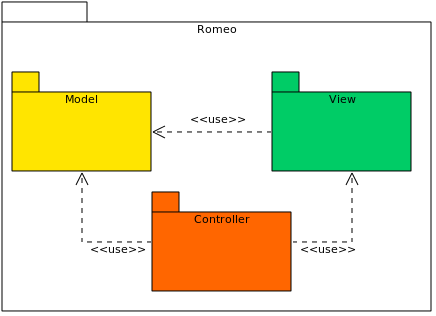
\includegraphics[scale=0.65] {../Specifica_Tecnica/Content/Immagini/Romeo.png}
			\caption{Componente Romeo}
			\label{romeoj}
\end{figure}

\section{Specifica componenti Romeo::Model}
\label{specificaModel}

\begin{figure} [!h]
\centering
	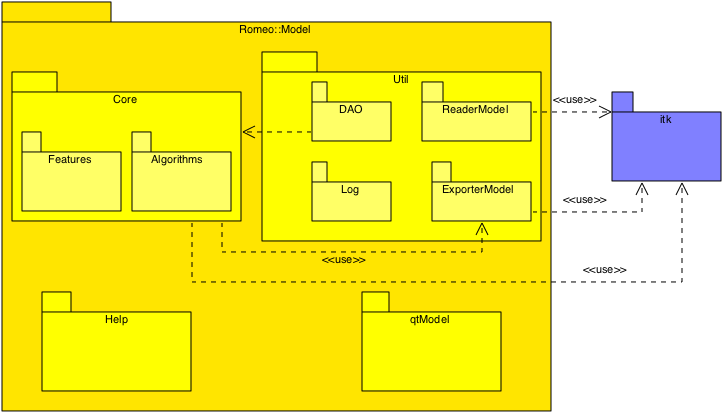
\includegraphics[scale=0.65] {../Specifica_Tecnica/Content/Immagini/Romeo__Model.png}
			\caption{Componente Romeo::Model}
			\label{comp_romeo_model}
\end{figure}

Package\g{} per il componente Model dell'architettura MVC.

\pagebreak
\subsection{Specifica componenti Model::Core}
\label{specifica_model_core}
\begin{figure}[!h]
\centering
			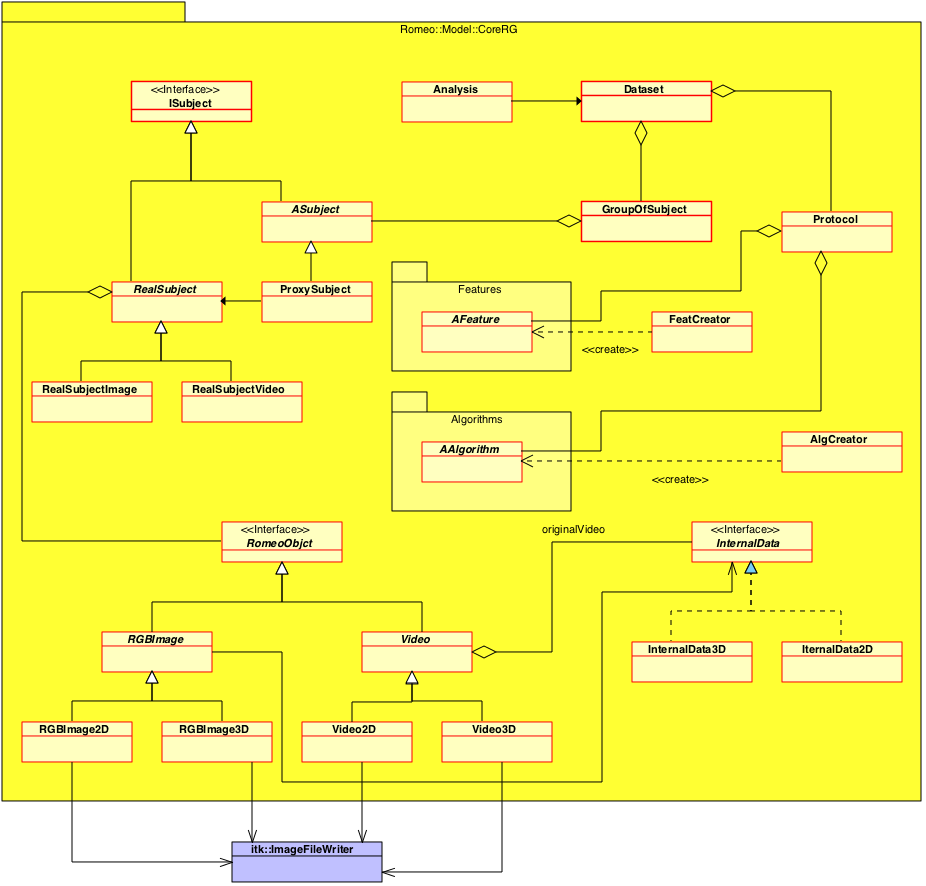
\includegraphics[scale=0.55]{../Specifica_Tecnica/Content/Immagini/Romeo__Model__Core.png}
			\caption{Diagramma package \textsl{Romeo::Model::Core}}
			\label{romeo_model_core}
\end{figure}
Package\g{} per il componente core.
% % % % % % % % % % % % % % % % % % % % % % % % % % % % % % % % % % %
% % ALGCREATOR % % % % % % % % % % % % % % % % % % % % % % % % % % % %
% % % % % % % % % % % % % % % % % % % % % % % % % % % % % % % % % % %

\subsubsection{AlgCreator (class)}
\label{algcreator}
	\begin{figure}[!h]
	\centering
				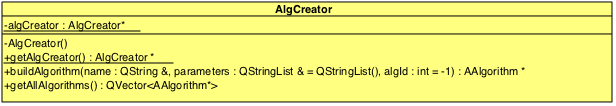
\includegraphics[scale=0.8]{./Content/Immagini/modelCore/AlgCreator.png}
				\caption{Diagramma classe \textsl{AlgCreator}}
				\label{algCreator_img}
	\end{figure}

	\paragraph{Descrizione\\}
	classe Factory avente la responsabilità di creare un oggetto di tipo \textsl{Romeo::Model::Core::Algorithms::AAlgorithm}, che rappresenta un' instanza dell' algoritmo da creare.
    \\Rappresenta il componente Factory del design pattern\g{} Factory.

	\paragraph{Utilizzo\\}
	viene utilizzata in seguito alla ricezione di un signal\g{} da parte dei controller che necessitano di utilizzare un oggetto di tipo \textsl{Romeo::Model::Core::Algorithms::AAlgorithm}.
	\\A seconda dei parametri e nome dell’ algoritmo di Cluster\g{} passati, crea un oggetto rispetto ad un altro.

	\paragraph{\textcolor{black}{Attributi\\}}
		\begin{itemize}
			\item \color{teal}\verb!- static algCreator: AlgCreator *!
			\color{black}
			\subparagraph{Descrizione:} puntatore all'unica istanza della classe \textsl{AlgCreator} che verrà creata in modo \textit{lazy} quando verrà richiesta la creazione dell'oggetto.
		\end{itemize}
		
\paragraph{\color{black}{Metodi}}
	\begin{itemize}
		%costruttore
		\item \color{blue}\verb! - AlgCreator()!
		\color{black}
		\subparagraph{Descrizione:} costruttore privato, come previsto dal design pattern\g{} Singleton.
		
		%getAlgCreator
		\item \color{blue}\verb! + static getAlgCreator : AlgCreator *!
		\color{black}
		\subparagraph{Descrizione:} metodo statico che  ritorna il puntatore all'unica istanza della classe \textsl{AlgCreator}. Nel caso in cui l'istanza non esista ancora, essa verrà creata e successivamente ritornata.
		\subparagraph{Note}
			\begin{itemize}
				\item Il metodo deve essere marcato come statico.
			\end{itemize}
			
		%buildAlgorithm
		\item \color{blue}\verb! + buildAlgorithm(name : const QString&, parameters : const QStringList& ,!
					\verb!algId : int) : AAlgorithm*!
		\color{black}
		\subparagraph{Descrizione:}Metodo che ha il compito di costruire l'algoritmo specificato, con i relativi parametri.\\
		Per esempio se il parametro \textit{name} è uguale a \lq\lq{}KMeans\rq\rq{} allora verrà creato un oggetto \textit{KMeansAlgorithm} con i dati passati nei parametri.
		\subparagraph{Argomenti}
			\begin{itemize}
				\item \color{RoyalPurple}\verb!name : const QString&!\\
				\color{black}Stringa che rappresenta il nome dell'algoritmo di clustering\g{} che si vuole creare;
				
				\item \color{RoyalPurple}\verb!parameters : const QStringList&!\\
				\color{black}Lista di stringhe che rappresenta i parametri da passare all'algoritmo di cluster\g{} che si vuole creare;
				
				\item \color{RoyalPurple}\verb!algId : int!\\
				\color{black}Rappresenta l'id da associare all'algorimo che si vuole creare. Nel caso non venga specificato assumerà il valore di default di \lq\lq{}-1\rq\rq{} che indica che l'algorimo non è già presente nel database.
			\end{itemize}
		\subparagraph{Note}
			\begin{itemize}
				\item Il metodo deve essere marcato come costante.
			\end{itemize}
	
	%getAllAlgorithms
	\item \color{blue}\verb! + getAllAlgorithms() : QVector<AAlgorithm *>!
	\color{black}
	\subparagraph{Descrizione:} metodo che ritorna tutte le possibili istanze di algoritmi di cluster\g{}.
	\subparagraph{Note}
		\begin{itemize}
			\item Il metodo deve essere marcato come costante.
		\end{itemize}
		
	\end{itemize}
	
\pagebreak
% % % % % % % % % % % % % % % % % % % % % % % % % % % %
% % ANALYSIS % % % % % % % % % % % % % % % % % % % % %
% % % % % % % % % % % % % % % % % % % % % % % % % % % % %
%\pagebreak
\color{black}
\subsubsection{Analysis (class)}
	\label{analysis}
	\begin{figure}[!h]
	\centering
				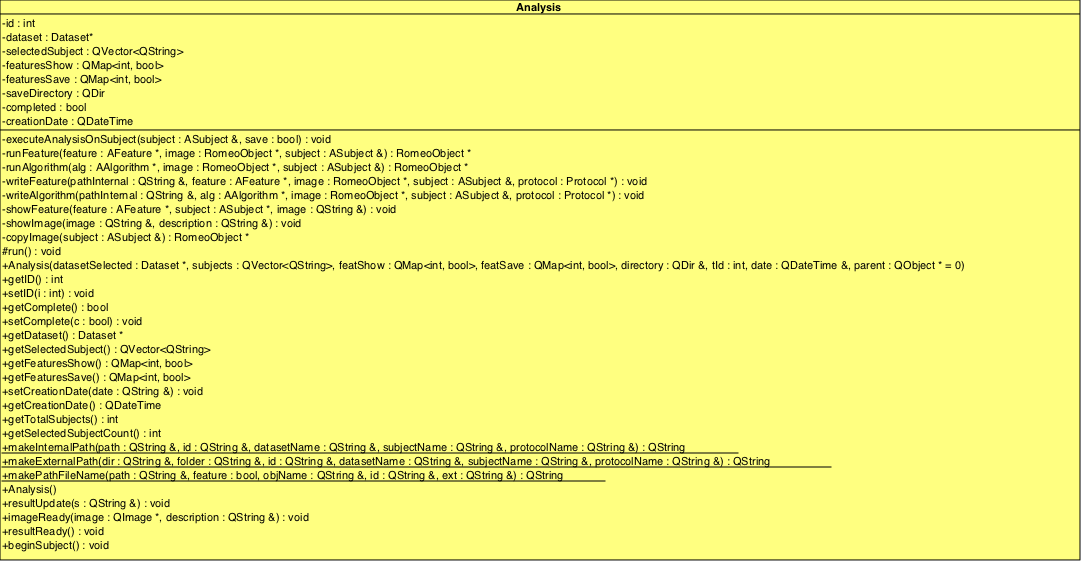
\includegraphics[scale=0.5]{./Content/Immagini/modelCore/Analysis.png}
				\caption{Diagramma classe \textsl{Analysis}}
				\label{analysis_img}
	\end{figure}

\paragraph{Descrizione \\}
classe che rappresenta un' analisi con le relative proprietà: \emph{Subject\g{} da analizzare, Directory dei risultati, Feature\g{} di cui salvare i risultati, Feature\g{} di cui visualizzare i risultati e Data di creazione}.
\\Rappresenta un Thread.

\paragraph{Utilizzo \\}
viene utilizzata dalla classe \textsl{AnalysisController}, alla ricezione di un signal\g{} per l'avvio di una nuova analisi.

\paragraph{Eredita da:}
	\begin{itemize}
		\item Qt::QThread.
	\end{itemize}
\paragraph{Attributi \\}
	\begin{itemize}
		\item \color{teal}\verb! - id : int!
		\color{black}
		\subparagraph{Descrizione:} rappresenta l'id associato all'analsi.
		
		\item \color{teal}\verb! - dataset!
		\color{black}
		\subparagraph{Descrizione:} puntatore all'oggetto \textsl{Dataset} associato all'analisi.
		
		\item \color{teal}\verb! - selectedSubject : QVector<QString>!
		\color{black}
		\subparagraph{Descrizione:} lista dei nomi dei Subject\g{} selezionati dall'utente su qui l'utente vuole eseguire l'analisi.
		
		\item \color{teal}\verb! - featuresShow : QMap<int, bool>!
		\color{black}
		\subparagraph{Descrizione:} mappa che rappresente le feature\g{} che l'utente vuole visualizzare nel dialogo.
		\\Ad ogni id delle feature è associato un \verb!bool! che indica se il risultato della feature\g{} deve essere visualizzata oppure no.
		
		\item \color{teal}\verb! - featuresSave : QMap<int, bool>!
		\color{black}
		\subparagraph{Descrizione:} mappa che rappresente le feature\g{} su cui l'utente vuole che siano esportati i risultati.
		\\Ad ogni id delle feature è associato un \verb!bool! che indica se il risultato della feature\g{} deve essere esportato oppure no.
		
		\item \color{teal}\verb! - saveDirectory : QDir!
		\color{black}
		\subparagraph{Descrizione:} cartella nel quale l'utente vuole che siano esportati i risultati.
		
		\item \color{teal}\verb! - completed : bool!
		\color{black}
		\subparagraph{Descrizione:} indica se l'analisi è terminata oppure no.
		
		\item \color{teal}\verb! - creationDate : QDateTime!
		\color{black}
		\subparagraph{Descrizione:} rappresenta la data in qui è stata avviata l'analisi.
			
	\end{itemize}

\color{black}
\paragraph{Metodi \\}
	\begin{itemize}
		%costruttore
		\item \color{blue}\verb! + Analysis(datasetSelected : Dataset *, subjects : QVector<QString>, !\\
								    \verb!featShow: const QMap<int, bool>, featSave : const QMap<int, bool>,!\\
							  		\verb! directory : const QDir&, tId : int, date : const QDateTime&, parent : QObject *);!\\
							  
		\color{black}
		\subparagraph{Descrizione:} costruttore della classe.
		
		\subparagraph{Argomenti:}
			\begin{itemize}
				\item \color{RoyalPurple}\verb!datasetSelected : Dataset *!\\
				\color{black}Puntatore al \textsl{Dataset} associato all'analisi;
				
				\item \color{RoyalPurple}\verb!subjects : QVector<QString>!\\
				\color{black}Lista dei nomi di Subject\g{} su qui eseguire l'analisi;
				
				\item \color{RoyalPurple}\verb!featShow: const QMap<int, bool>!\\
				\color{black}Mappa che associa ad un id di una feature\g{} un \verb!bool! che indica se la il risultato della feature\g{} va visualizzato nel dialogo oppure no;
				
				\item \color{RoyalPurple}\verb!featSave : const QMap<int, bool>!\\
				\color{black}Mappa che associa ad un id di uan feature\g{} un \verb!bool! che indica se il risultato della feature\g{} va esportato oppure no;
				
				\item \color{RoyalPurple}\verb!directory : const QDir&!\\
				\color{black}Directory nel quale salvare i risultati delle feature\g{} e degli algoritmi di clustering\g{};
				
				\item \color{RoyalPurple}\verb!tId : int!\\
				\color{black}Id associato all'analisi. Di default vale \lq\lq{}-1\rq\rq{};
				
				\item \color{RoyalPurple}\verb! date : const QDateTime&!\\
				\color{black}Data nel quale è stata creata l'analisi;
				
				\item \color{RoyalPurple}\verb!parent : QObject *!\\
				\color{black}Parente dell'oggetto Analysis.
			\end{itemize}
			
	\item \color{blue}\verb! - executeAnalysisOnSubject(subject : ASubject&, save : bool) : void!\\
	\color{black}\subparagraph{Descrizione:} metodo che esegue l'intera analisi sul \textsl{Subject} passato.
	\subparagraph{Argomenti}
		\begin{itemize}
			\item \color{RoyalPurple}\verb!subject : ASubject&!\\
			\color{black}Subject su qui eseguire l'analisi;
			
			\item \color{RoyalPurple}\verb!save : bool!\\
			\color{black}Booleano che indica se i risultati delle feature\g{} e degli algoritmi di clustering\g{} devono essere salvati o meno.
		\end{itemize}
	
	\item \color{blue}\verb! - runFeature(feature : AFeature *, image : RomeoObject *, !\\
	                            \verb!subject : ASubject &) : RomeoObject *!\\
	\color{black}\subparagraph{Descrizione:} metodo che esegue una feature\g{} sul formato interno dell'immagine passato come parametro.
	\\Ritorna un \textsl{RomeoObject *} rappresentante il formato interno dell'immagine di output.
	\subparagraph{Argomenti}
		\begin{itemize}
			\item \color{RoyalPurple}\verb!feature : AFeature *!\\
			\color{black}Feature da eseguire;
			
			\item \color{RoyalPurple}\verb!image : RomeoObject *!\\
			\color{black}Formato interno su cui eseguire la feature\g{};
			
			\item \color{RoyalPurple}\verb!subject : ASubject &!\\
			\color{black}Rappresenta il \textsl{Subject} su cui eseguire l'analisi.
		\end{itemize}
		
	\item \color{blue}\verb!- runAlgorithm(alg : AAlgorithm *, image : RomeoObject *, !\\
	                            \verb!subject : ASubject &) : RomeoObject *!\\
	\color{black}\subparagraph{Descrizione:} metodo che esegue un algoritmo\g{} sul formato interno dell'immagine passato come parametro.
	\\Ritorna un \textsl{RomeoObject *} rappresentante il formato interno dell'immagine di output.
	\subparagraph{Argomenti}
		\begin{itemize}
			\item \color{RoyalPurple}\verb!alg : AAlgorithm *!\\
					\color{black}Algoritmo da eseguire;
					
			\item \color{RoyalPurple}\verb!image : RomeoObject *!\\
			\color{black}Formato interno su cui eseguire la feature\g{};
		
			\item \color{RoyalPurple}\verb!subject : ASubject &!\\
			\color{black}Rappresenta il \textsl{Subject} su cui eseguire l'analisi.
		\end{itemize}
		
	\item \color{blue}\verb! - writeFeature(pathInternal : const QString&, !\\
								\verb!feature : AFeature*, image : RomeoObject *,subject : ASubject &,!\\
								\verb!protocol : Protocol *) : void!\\
			\color{black}\subparagraph{Descrizione:} metodo che esporta il risultato della feature\g{} nel filesystem.
			\subparagraph{Argomenti}
				\begin{itemize}
					\item \color{RoyalPurple}\verb!pathInternal : const QString&!\\
					\color{black}Path nel quale salvare il risultato della feature\g{};
					
					\item \color{RoyalPurple}\verb!feature : AFeature*!\\
					\color{black}Rappresenta la feature\g{} che è appena stata eseguita;
					
					\item \color{RoyalPurple}\verb!image : RomeoObject *!\\
					\color{black}Rappresenta il formato interno dell'imamgine che va esportata;
					
					\item \color{RoyalPurple}\verb!subject : ASubject &!\\
					\color{black}Rappresenta il Subject\g{} sul quale è stata eseguita la feature\g{};
					
					\item \color{RoyalPurple}\verb!protocol : Protocol *!\\
					\color{black}Rappresenta il Protocol\g{} al quale appartiene la Feature\g{} appena eseguita.
				\end{itemize}
				
		
	\item \color{blue}\verb! - writeAlgorithm(pathInternal : const QString&,!\\
	 						    \verb! alg : AAlgorithm*, image : RomeoObject *,!\\
									\verb! subject : ASubject &, protocol : Protocol *) : void!\\
				\color{black}\subparagraph{Descrizione:} metodo che esporta il risultato dell'algoritmo di clustering\g{} nel filesystem.
				\subparagraph{Argomenti}
					\begin{itemize}
						\item \color{RoyalPurple}\verb!pathInternal : const QString&!\\
						\color{black}Path nel quale salvare il risultato dell'algoritmo\g{};
						
						\item \color{RoyalPurple}\verb!alg : AAlgorithm*!\\
						\color{black}Rappresenta l'algoritmo di clustering\g{} che è appena stato eseguito;
						
						\item \color{RoyalPurple}\verb!image : RomeoObject *!\\
						\color{black}Rappresenta il formato interno dell'imamgine che va esportata;
						
						\item \color{RoyalPurple}\verb!subject : ASubject &!\\
						\color{black}Rappresenta il Subject\g{} sul quale è stato eseguito l'algorimo di clustering\g{};
						
						\item \color{RoyalPurple}\verb!protocol : Protocol *!\\
						\color{black}Rappresenta il Protocol\g{} al quale appartiene l'algoritmo di clustering\g{} appena eseguito.
					\end{itemize}
	
	\item \color{blue}\verb! - showFeature(feature : AFeature *, subject : ASubject *,!\\
						       \verb! image : const QString &) : void!\\
			 \color{black}\subparagraph{Descrizione:} metodo che si occupa di creare un oggetto \verb!QImage! sul risultato di una feature\g{}.
			 \subparagraph{Argomenti}
			 	\begin{itemize}
				 	\item \color{RoyalPurple}\verb!feature : AFeature *!\\
				 	\color{black}Rappresenta la feature\g{} che è stata eseguita;
				 	
				 	\item \color{RoyalPurple}\verb!subject : ASubject *!\\
				 	\color{black}Rappresenta il Subject\g{} su cui è stata eseguita la feature\g{};
				 	
				 	\item \color{RoyalPurple}\verb!image : const QString &!\\
				 	\color{black}Percorso nel quale è presente il risultato della feature\g{} appena eseguita.
			 	\end{itemize}
	
	\item \color{blue}\verb! - showImage(image : const QString &, type : const QString &,!\\
								\verb! description : const QString &) : void!\\
	\color{black}\subparagraph{Descrizione:}  metodo che emette il signal\g{} \verb!imageReady! quando un algoritmo di clustering\g{} o una feature\g{} è terminata.
	\subparagraph{Argomenti}
		\begin{itemize}
			\item \color{RoyalPurple}\verb!image : const QString &!\\
			\color{black}Rappreenta il percorso nel quale si trova l'immagine risultato;
			
			\item \color{RoyalPurple}\verb!type : const QString &!\\
			\color{black}Rappresenta il tipo di immagine;
			
			\item \color{RoyalPurple}\verb!description : const QString &)!\\
			\color{black}Rappresenta la descrizione dell'immagine.
		\end{itemize}
		
	\item \color{blue}\verb! + run() : void!\\
	\color{black}\subparagraph{Descrizione:} avvia il thread.
	\subparagraph{Note}
		\begin{itemize}
			\item Il metodo deve essere marcato come virtuale.
		\end{itemize}
	
	\item \color{blue}\verb! + getID() :int!\\
	\color{black}\subparagraph{Descrizione:} metodo che ritorna l'id associato all'istanza.
	\subparagraph{Note}
		\begin{itemize}
			\item Il metodo deve essere marcato costante.
		\end{itemize}
		
	\item \color{blue}\verb! + setID(i : int) : void!\\
	\color{black}\subparagraph{Descrizione:} cambia l'id associato all'oggetto \textsl{Analysis}.
	\subparagraph{Argomenti}
		\begin{itemize}
			\item \color{RoyalPurple}\verb!i : int!\\
			\color{black}Il nuovo id da associare.
		\end{itemize}
		
	\item \color{blue}\verb! + getComplete() : bool!\\
	\color{black}\subparagraph{Descrizione:} ritorna un \verb!bool! che indica se l'analisi è stata terminata o meno.
	\subparagraph{Note}
		\begin{itemize}
			\item Il metodo deve essere marcato come costante.
		\end{itemize}
		
	\item \color{blue}\verb! + setComplete(c : bool) : void!\\
	\color{black}\subparagraph{Descrizione:} metodo che cambia lo stato di completamento dell'analisi.
	\subparagraph{Argomenti}
		\begin{itemize}
			\item \color{RoyalPurple}\verb!c : bool!\\
			Rappresenta il nuovo stato di completamento dell'analsi.
		\end{itemize}
		
	\item \color{blue}\verb!+ getDataset() : Dataset*!\\
	\color{black}\subparagraph{Descrizione:} metodo che ritorna l'oggetto \textsl{Dataset} associato all'analisi.
	\subparagraph{Note}
		\begin{itemize}
			\item Il metodo deve essere marcato come costante.
		\end{itemize}
		
	\item \color{blue}\verb! + getSelectedSubject() : QVector<QString>!\\
	\color{black}\subparagraph{Descrizione:} metodo che ritorna la lista dei Subject\g{} su cui eseguire l'analisi.
	\subparagraph{Note}
		\begin{itemize}
			\item Il metodo deve essre marcato come costante.
		\end{itemize}
		
	\item \color{blue}\verb! + getFeaturesShow() : QMap<int, bool>!\\
	\color{black}\subparagraph{Descrizione:} metodo che ritorna una \verb! QMap! che associa all'id di una feature un \verb!bool! che indica se il risultato della feature\g{} va visualizzati nel dialogo oppure no.
	\subparagraph{Note}
		\begin{itemize}
			\item Il metodo deve essere marcato come costante.
		\end{itemize}
		
	\item \color{blue}\verb! +  getFeaturesSave() :QMap<int, bool>!\\
	\color{black}\subparagraph{Descrizione:} metodo che ritorna una \verb! QMap! che associa all'id di una feature un \verb!bool! che indica se il risultato della feature\g{} va esportato oppure no.
		\subparagraph{Note}
			\begin{itemize}
				\item Il metodo deve essere marcato come costante.
			\end{itemize}
			
	\item \color{blue}\verb! + setCreationDate(date : const QString &) : void!\\
	\color{black}\subparagraph{Descrizione:} metodo che cambia la data di creazione di un oggetto \textsl{Analysis}.
	\subparagraph{Argomenti}
		\begin{itemize}
			\item \color{RoyalPurple}\verb!date : const QString &!\\
			\color{black}Nuova data di creazione.
		\end{itemize}
		
	\item \color{blue}\verb! + getCreationDate() : QDateTime!\\
	\color{black}\subparagraph{Descrizione:} metodo che ritorna la data di creazione di un oggetto \textsl{Analysis}.
	\subparagraph{Note}
	\begin{itemize}
		\item Il metodo va marcato come costante.
	\end{itemize}
	
	\item \color{blue}\verb! + getTotalSubjects() :int!\\
	\color{black}\subparagraph{Descrizione:} metodo che ritorna il numero di Subject\g{} presenti nel Gruppo di Subject associati al Dataset\g{} dell'analisi.
	\subparagraph{Note}
		\begin{itemize}
			\item Il metodo deve essere marcato costante.
		\end{itemize}
		
	\item \color{blue}\verb! + getSelectedSubjectCount() : int!\\
	\color{black}\subparagraph{Descrizione:} metodo che ritorna il numero di Subject\g{} su cui eseguire l'analisi.
	\subparagraph{Note}
		\begin{itemize}
			\item Il metodo deve essere marcato costante.
		\end{itemize}
		
	\item \color{blue}\verb! + resultUpdate(s : const QString &) : void (signal)!\\    
	\color{black}\subparagraph{Descrizione:} signal\g{} emesso quando va aggiornata la descrizione dell'oggetto \textsl{AnalysisDialog}.
	\subparagraph{Argomenti}
		\begin{itemize}
			\item \color{RoyalPurple}\verb!s : const QString &!\\
			\color{black}Nuovo testo da visualizzare nel dialogo.
		\end{itemize}   
		
	\item \color{blue}\verb! + imageReady(image : QImage *, description : const QString &) : void (signal)!\\
	\color{black}\subparagraph{Descrizione:} signal\g{} emesso quando una nuova immagine è disponibile.
	\subparagraph{Argomenti}
		\begin{itemize}
			\item \color{RoyalPurple}\verb!image : QImage *!\\
			\color{black}Nuova immagine disponibile;
			
			\item \color{RoyalPurple}\verb!description : const QString &!\\
			\color{black}Descrizione associata all'immagine.
		\end{itemize}
		
	\item \color{blue}\verb! + resultReady() : void (signal)!\\
	\color{black}\subparagraph{Descrizione:} signal\g{} emesso quando l'esecuzione dell'analisi è terminata.
	
	\item \color{blue}\verb! +beginSubject() : void (signal)!\\
	\color{black}\subparagraph{Descrizione:} signal\g{} emesso quando l'analisi viene effettuata su un nuovo Subject\g{}.

	\end{itemize}
 


\pagebreak
% % % % % % % % % % % % % % % % % % % % % % % % % % % % % 
% % ISubject & % % % % % % % % % % % % % % % % % % % % %
% % % % % % % % % % % % % % % % % % % % % % % % % % % % %
\color{black}
\subsubsection{ISubject (interface)}
\label{iSubject}
\begin{figure}[!h]
\centering
			\centering
			 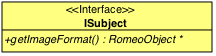
\includegraphics[scale=1.00]{./Content/Immagini/modelCore/ISubject.png}
			 \caption{Diagramma classe \textsl{ISubject}}
			\label{iSubject_img}
\end{figure}

\paragraph{Descrizione \\}
	Definisce l’interfaccia comune per le classi \textsl{ASubject} e \textsl{RealSubjec}, fornisce un metodo per ottenere il formato interno per l’immagine del Subject\g{}.
	\\Rappresenta il componente Subject del design pattern\g{} Proxy.

\paragraph{Utilizzo \\}
Viene utilizzata quando le componenti di Romeo\g{} necessitano di riferirsi a un Subject\g{} per ottenere il formato interno ad esso associato. 

\paragraph{\color{black}Metodi}
\begin{itemize}
			\item \color{blue} \verb!+ getImageFormat() : RomeoObject *!
			\color{black}
			\subparagraph{Descrizione:} contratto che restituisce un puntatore al formato interno dell'immagine di un Subject\g{}
			\subparagraph{Note}
			\begin{itemize}
				\item Il metodo deve essere marcato come virtuale.
			\end{itemize}
\end{itemize}
\pagebreak
% % % % % % % % % % % % % % % % % % % % % % % % % % % % % 
% % ASubject & % % % % % % % % % % % % % % % % % % % % %
% % % % % % % % % % % % % % % % % % % % % % % % % % % % %
\color{black}
\subsubsection{ASubject (abstract)}
\label{aSubject}
\begin{figure}[!h]
\centering
			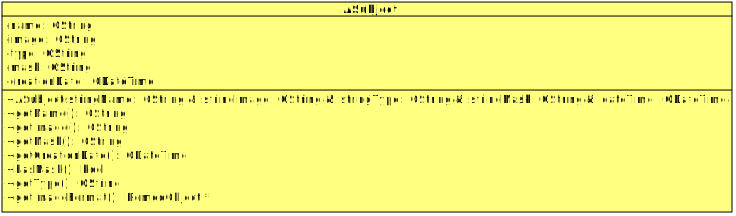
\includegraphics[scale=0.80]{./Content/Immagini/modelCore/ASubject}
			\caption{Diagramma classe \textsl{ASubject}}
			\label{aSubject_img}
\end{figure}

\paragraph{Descrizione \\}
Classe astratta che rappresenta un generico Subject\g{} con le relative proprietà \emph{Nome, Tipo del Subject\g{}, Immagine, Maschera e Data di creazione}.

\paragraph{Utilizzo \\}
 Viene utilizzata in seguito alla ricezione di un signal\g{} da parte dei controller che necessitano di riferirsi ad uno o più oggetti di tipo \textsl{ASubject}.
 \\Inoltre viene utilizzata dalle classi DAO e dalla classe \textsl{GroupOfSubject}.
 
\paragraph{Eredita da:}
\begin{itemize}
	\item Romeo::Model::Core::ISubject: non implementa ancora i contratti di questa classe.
\end{itemize}

\paragraph{Attributi \\}
	\begin{itemize}
			\item \color{teal} \verb!- name : QString!
					\color{black}
					\subparagraph{Descrizione:} nome del Subject\g{}.
					\item \color{teal} \verb!- image : QString!
					\color{black}
					\subparagraph{Descrizione:} stringa rappresentante il percorso assoluto dell'immagine del Subject\g{}.
					\item \color{teal} \verb!- type : QString!
					\color{black}
					\subparagraph{Descrizione:} stringa rappresentante il tipo di un Subject\g{} (2D, 2D-t, 3D, 3D-t).
					\item \color{teal} \verb!- mask : QString!
					\color{black}
					\subparagraph{Descrizione} stringa rappresentante il percorso della maschera del Subject\g{}.
					\item \color{teal} \verb!- creationDate : QDateTime!
					\color{black}
					\subparagraph{Descrizione:} data di creazione del Subject\g{}
	\end{itemize}
	
\paragraph{\color{black}Metodi \\}
\begin{itemize}

			%Costruttore
			\item \color{blue} \verb!+ ASubject(stringName : const QString &, stringImage : const QString &,!
			\verb!stringType : const QString &, stringMask : const QString &, dateTime : const QDateTime &)!
			\color{black}
			\subparagraph{Descrizione:} costruttore della classe.
			\color{black}
			\subparagraph{Argomenti}
				\begin{itemize}
					\item \color{RoyalPurple} \verb!stringName : const QString &!\\				
								\color{black} Nome del Subject\g{}.
					\item \color{RoyalPurple} \verb!stringImage : const QString &!\\				
								\color{black} Percorso dell'immagine del Subject\g{};
					\item \color{RoyalPurple} \verb!stringType : const QString &!\\				
								\color{black} Stringa che rappresenta il tipo del Subject\g{} (2D, 2D-t, 3D, 3D-t).
					\item \color{RoyalPurple} \verb!stringMask : const QString &!\\				
							  \color{black} Stringa rappresentante il percorso della maschera del Subject\g{}.
					\item \color{RoyalPurple} \verb!dateTime : const QDateTime &!\\				
								\color{black} Data di creazione del Subject\g{}.
				\end{itemize}
			
			%getName	
			\item \color{blue} \verb!+ getName() : QString! 
			\color{black}
			\subparagraph{Descrizione:} metodo che ritorna una stringa, contenente il nome del Subject\g{}.
			\subparagraph{Note}
			\begin{itemize}
				\item Il metodo deve essere marcato costante.
			\end{itemize}
			
			%getImage
			\item \color{blue} \verb!+ getImage() : QString! 
			\color{black}
			\subparagraph{Descrizione:} metodo che ritorna una stringa, contenete il percorso assoluto dell'immagine associata al Subject\g{}.
			\subparagraph{Note}
			\begin{itemize}
				\item Il metodo deve essere marcato costante.
			\end{itemize}
			
			%getMask
			\item \color{blue} \verb!+ getMask() : QString! 
			\color{black}
			\subparagraph{Descrizione:} metodo che ritorna una stringa, contente il percorso assoluto della (eventuale) maschera associata al Subject\g{}.
			\subparagraph{Note}
			\begin{itemize}
				\item Il metodo deve essere marcato costante.
			\end{itemize}
			
			%getCreationDate
			\item \color{blue} \verb!+ getCreationDate() : QDateTime!
			\color{black}
			\subparagraph{Descrizione:} metodo che ritorna la data di creazione del Subject\g{}.
			\subparagraph{Note}
			\begin{itemize}
				\item Il metodo deve essere marcato costante.
			\end{itemize}
			
			%hasMask
			\item \color{blue} \verb!+ hasMask() : bool!
			\color{black}
			\subparagraph{Descrizione:} metodo che controlla se il Subject\g{} contiene una maschera\g{} oppure no.
			\\Ritorna \verb!true! se il Subject\g{} possiede una maschera, \verb!false! viceversa.
			\subparagraph{Note}
			\begin{itemize}
				\item Il metodo deve essere marcato costante.
			\end{itemize}
			
			%getType
			\item \color{blue} \verb!+ getType() : QString!
			\color{black}
			\subparagraph{Descrizione} Metodo che ritorna una stringa, contente il tipo del Subject\g{} (2D, 2-t, 3D, 3D-t).
			\subparagraph{Note}
			\begin{itemize}
				\item Il metodo deve essere marcato const.
			\end{itemize}
		\end{itemize}


% % % % % % % % % % % % % % % % % % % % % % % % % % % % % 
% % ProxySubject & % % % % % % % % % % % % % % % % % % % % %
% % % % % % % % % % % % % % % % % % % % % % % % % % % % %
\pagebreak
\color{black}
\subsubsection{ProxySubject (class)}
\label{proxySubject}
\begin{figure}[!h]
\centering
			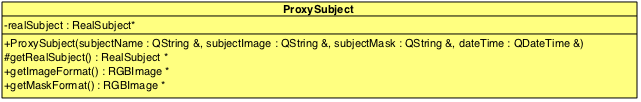
\includegraphics[width=1\linewidth]{./Content/Immagini/modelCore/ProxySubject.png}
			\caption{Diagramma classe \textsl{ProxySubject}}
			\label{proxySubject_img}
\end{figure}

\paragraph{Descrizione \\}
Classe che gestisce l’accesso ad un \textsl{RealSubject}, mantiene un riferimento che consente al proxy di accedere all’oggetto rappresentato \textsl{RealSubject}.
\\Fornisce la stessa interfaaccia della classe \textsl{ASubject}, consentendo di utilizzare un oggetto \textsl{ProxySubject} quando è richiesto un oggetto \textsl{ASubject}.
\\Rappresenta il componente Proxy del design pattern\g{} Proxy.

\paragraph{Utilizzo \\}
Viene utilizzando quando è necessario creare un Subject\g{} all'interno di Romeo\g{}.

\paragraph{Eredita da:}
\begin{itemize}
	\item Romeo::Model::Core::ISubject: implementa i contratti di questa classe.
\end{itemize}

\paragraph{Attributi \\}
	\begin{itemize}
		\item \color{teal}\verb! - realSubject : RealSubject *!
		\color{black}
		\subparagraph{Descrizione:} puntatore ad un oggetto di tipo \textsl{RealSubject} che il Proxy sta rappresentando.
	\end{itemize}

\color{black}
\paragraph{Metodi \\}
	\begin{itemize}
		%costruttore
		\item  \color{blue}\verb! + ProxySubject(subjectName : const QString&, subjectImage : const QString&, !\\
			\verb!maskName : const QString&, dateTime : const QDateTime&)!
			\color{black}
			\subparagraph{Descrizione:} costruttore della classe. Richiama il costruttore della superclasse.
			\subparagraph{Argomenti}
				\begin{itemize}
					\item \color{RoyalPurple}\verb!subjectName : const QString&!\\
					\color{black}Nome del Subject\g{}. Viene passato al costruttore della superclasse;
					
					\item \color{RoyalPurple}\verb!subjectImage : const QString&!\\
					\color{black}Immagine del Subject\g{}. Viene passato al costruttore della superclasse;
					
					\item \color{RoyalPurple}\verb!maskName : const QString&!\\
					\color{black}Maschera\g{} del \subject{}. Viene passato al costruttore della superclasse;
					
					\item \color{RoyalPurple}\verb!dateTime : QDateTime &!\\
					\color{black}Data di creazione del \subject{}. Viene passato al costruttore della superclasse.
				\end{itemize}
		
		%getRealSubject
		\item \color{blue}\verb! # getRealSubject() : RealSubject *!
		\color{black}
		\subparagraph{Descrizione:} restituisce il puntatore al \textsl{RealSubject} rappresentato. Nel caso non esista viene creato e successivmente ritornato.
		
		%getImageFormat
		\item \color{blue}\verb! + getImageFormat() : RomeoObject *!
		\color{black}
		\subparagraph{Descrizione:} Implementa il contratto fornito dalla superclasse. Si limita a chiamare il metodo \verb!getImageFormat()! sull'oggetto \textsl{RealSubject}.
		
		\subparagraph{Note}
			\begin{itemize}
				\item Il metodo deve essere marcato virtuale.
			\end{itemize}
			
	\end{itemize}


\pagebreak
% % % % % % % % % % % % % % % % % % % % % % % % % % % % % 
% % RealSubject & % % % % % % % % % % % % % % % % % % % % %
% % % % % % % % % % % % % % % % % % % % % % % % % % % % %
\color{black}
\subsubsection{RealSubject (abstract)}
\label{RealSubject}
\begin{figure}[!h]
\centering
			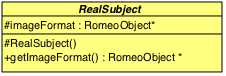
\includegraphics[scale=1]{./Content/Immagini/modelCore/RealSubject.png}
			\caption{Diagramma classe \textsl{RealSubject}}
			\label{realSubject_img}
\end{figure}

\paragraph{Descrizione \\}
classe astratta che caratterizza l’oggetto rappresentato dal \textsl{ProxySubject}, rappresenta un oggetto reale utilizzato dalla classe \textsl{ProxySubject}.
\\Contiene la proprietà \emph{imageFormat}.
\\Le sottoclassi rappresentano i componenti RealSubject del design pattern\g{} Proxy.

\paragraph{Utilizzo \\}
 viene utilizzato dalla classe \textsl{ProxySubject}, la quale contiene un riferimento al \textsl{RealSubject} che sta gestendo.
 
\paragraph{Eredita da:}
\begin{itemize}
	\item Romeo::Model::Core::ISubject: implementa i contratti di questa classe.
\end{itemize}

\paragraph{Attributi}
	\begin{itemize}
	   %imageFormat
		\item \color{teal}\verb! # imageFormat : RomeoObject *!
		\color{black}
		\subparagraph{Descrizione:} puntatore al formato interno utilizzato per rappresentare l'immagine associata al Subject\g{}.
	\end{itemize}

\paragraph{\color{black}Metodi}
	\begin{itemize}
		%costruttore
		\item \color{blue}\verb! # RealSubject()!
		\color{black}
		\subparagraph{Descrizione:} costruttore della classe. Il costruttore è stato reso protetto in quanto la classe è ancora astratta.
	\end{itemize}

\pagebreak
% % % % % % % % % % % % % % % % % % % % % % % % % % % % % 
% % RealSubjectImage & % % % % % % % % % % % % % % % % % % % % %
% % % % % % % % % % % % % % % % % % % % % % % % % % % % %
\color{black}
\subsubsection{RealSubjectImage (class)}
\label{RealSubject2D}
\begin{figure}[!h]
\centering
			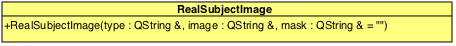
\includegraphics[scale=1]{./Content/Immagini/modelCore/RealSubjectImage.png}
			\caption{Diagramma classe \textsl{RealSubjectImage}}
			\label{realSubject2d_img}
\end{figure}

\paragraph{Descrizione \\}
Classe concreta che rappresenta un Subject\g{} nel formato bidimensionale (2D, 3D).

\paragraph{Utilizzo \\}
Viene utilizzata dalla classe \textsl{ProxySubject} per ottenere l'oggetto di tipo \textsl{RomeoObject} che rappresenta l'immagine, quando il \textsl{ProxySubject} sta rappresentando un Subject\g{} 2D o 3D.

\paragraph{Eredita da:}
\begin{itemize}
	\item Romeo::Model::Core::RealSubject.
\end{itemize}

\paragraph{Metodi \\}
	\begin{itemize}
		\item \color{blue}\verb! + RealSubjectImage(image : const QString &, mask : const QString &)!
		\color{black}
		\subparagraph{Descrizione:} costruttore della classe. Richiama il costruttore della supeclasse.
		\\Rappresenta il componente RealSubject del design pattern\g{} Proxy.
		
		\subparagraph{Argomenti}
			\begin{itemize}
				\item \color{RoyalPurple}\verb!image : const QString &!\\
				\color{black}Stringa che rappresenta il path nel quale è presente l'immagine del Subject\g{};
				
				\item \color{RoyalPurple}\verb!mask : const QString &)!\\
				\color{black}Stringa che rappresenta il path nel quale è presente la maschera del Subject\g{}.
				Nel caso in qui il Subject\g{} non abbia alcuna maschera l'argomento \verb!mask! assumerà il valore di default "".
			\end{itemize}
	\end{itemize}

\pagebreak
% % % % % % % % % % % % % % % % % % % % % % % % % % % % % 
% % RealSubjectVideo & % % % % % % % % % % % % % % % % % % % % %
% % % % % % % % % % % % % % % % % % % % % % % % % % % % %
\color{black}
\subsubsection{RealSubjectVideo (class)}
\label{RealSubject3D}
\begin{figure}[!h]
\centering
			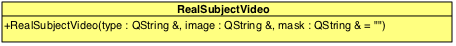
\includegraphics[scale=1]{./Content/Immagini/modelCore/RealSubjectVideo.png}
			\caption{Diagramma classe \textsl{RealSubjectVideo}}
			\label{realSubject3d_img}
\end{figure}

\paragraph{Descrizione \\}
Classe concreta che rappresenta un Subject\g{} di tipo 2D-t o 3D-t.
\\Rappresenta il componente RealSubject del design pattern\g{} proxy.

\paragraph{Utilizzo \\}
Viene utilizzata dalla classe \textsl{ProxySubject} per ottenere l'oggetto di tipo \textsl{RomeoObject} che rappresenta l'immagine, quando il \textsl{ProxySubject} sta rappresentando un Subject\g{} 2D-t o 3D-t.
			

\paragraph{Eredita da:}
\begin{itemize}
	\item Romeo::Model::Core::RealSubject.
\end{itemize}

\paragraph{Metodi \\}
\begin{itemize}
		\item \color{blue}\verb! + RealSubjectVideo(image : const QString &, mask : const QString &)!
		\color{black}
		\subparagraph{Descrizione:} costruttore della classe. Richiama il costruttore della supeclasse.
		\\Rappresenta il componente RealSubject del design pattern\g{} Proxy.
		
		\subparagraph{Argomenti}
			\begin{itemize}
				\item \color{RoyalPurple}\verb!image : const QString &!\\
				\color{black}Stringa che rappresenta il path nel quale è presente l'immagine del Subject\g{};
				
				\item \color{RoyalPurple}\verb!mask : const QString &)!\\
				\color{black}Stringa che rappresenta il path nel quale è presente la maschera del Subject\g{}.
				Nel caso in qui il Subject\g{} non abbia alcuna maschera l'argomento \verb!mask! assumerà il valore di default "".
			\end{itemize}
	\end{itemize}

\pagebreak
% % % % % % % % % % % % % % % % % % % % % % % % % % % % % 
% % GroupOfSubject % % % % % % % % % % % % % % % % % % % % %
% % % % % % % % % % % % % % % % % % % % % % % % % % % % %
\color{black}
\subsubsection{GroupOfSubject (class)}
\label{groupOfSubject}
\begin{figure}[!h]
\centering
			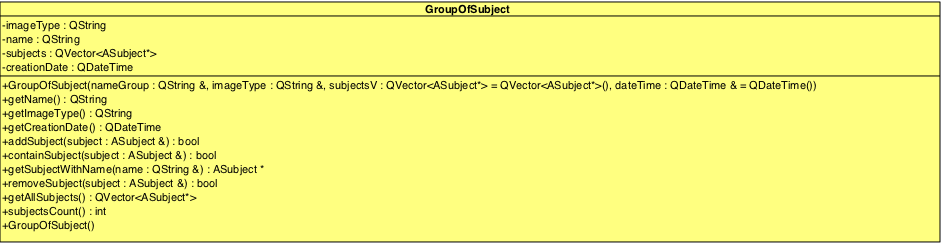
\includegraphics[width=1.2\linewidth]{./Content/Immagini/modelCore/GroupOfSubject.png}
			\caption{Diagramma classe \textsl{GroupOfSubject}}
			\label{groupOfSubject_img}
\end{figure}

\paragraph{Descrizione \\}
Classe che rappresenta un gruppo di Subject\g{} con le relative propietà: \emph{Nome del gruppo, tipo del gruppo, data di creazione e la lista di Subject\g{} presenti nel gruppo}.

\paragraph{Utilizzo \\}
Viene utilizzata in seguito alla ricezione di un signal\g{} da parte dei controller che necessitano di riferirsi ad uno o più gruppi di Subject\g{}
\\Inoltre viene utilizzata dalla classe \textsl{Dataset}, che contiene un riferimento al GroupOfSubject\g{} associato e dalle classi DAO.

\paragraph{Attributi }
	\begin{itemize}
		\item \color{teal}\verb!- imageType : QString!
		\color{black}\subparagraph{Descrizione:} stringa rappresentante il tipo del gruppo.
		
		% name
		
		\item \color{teal}\verb!- name : QString !
		\color{black}\subparagraph{Descrizione:} nome del gruppo.
			
		% mask
		\item \color{teal}\verb!- subjects : QVector<ASubject*> !
			\color{black}\subparagraph{Descrizione:} vettore di puntatori ad \textsl{ASubject} contenente i \subject{} facenti parte del gruppo.

		% creationDate
		\item \color{teal}\verb!- creationDate : QDateTime !
			\color{black}\subparagraph{Descrizione:} data di creazione del gruppo.
	\end{itemize}
	
\paragraph{Metodi \\}
	\begin{itemize}
		\item \color{blue}\verb! + GroupOfSubject(nameGroup : const QString&, imageType : const QString&,!\\
									 \verb! subjectsV : QVector<ASubject*>  ,  dateTime : const QDateTime&)!\\
				\color{black}
					\subparagraph{Descrizione:} costruttore della classe \textsl{GroupOfSubjcect}.
					\subparagraph{Argomenti}
						\begin{itemize}
							\item \color{RoyalPurple}\verb!nameGroup : const QString&!\\
							\color{black}Nome del Gruppo di Subject\g{};
							
							\item \color{RoyalPurple}\verb!imageType : const QString&!\\
							\color{black}Tipo del Gruppo di Subject\g{ (2D, 2D-t, 3D, 3D-t)};
							
							\item \color{RoyalPurple}\verb!subjectsV : QVector<ASubject*>!\\
							\color{black}Subject\g{} presenti nel gruppo;
							
							\item \color{RoyalPurple}\verb!dateTime : const QDateTime&!\\
							\color{black}Data di creazione del Subject\g{}.
						\end{itemize}
						
		\item \color{blue}\verb! + getName() : QString !\\
		\color{black}
		\subparagraph{Descrizione:} ritorna una stringa contenente il nome del gruppo.
		\subparagraph{Note}
			\begin{itemize}
				\item Il metodo deve essere marcato come costante.
			\end{itemize}
			
		
		\item \color{blue}\verb! + getImageType() : QString !\\
		\color{black}
		\subparagraph{Descrizione:} ritorna una stringa contenente il percorso del gruppo.
		\subparagraph{Note}
			\begin{itemize}
				\item Deve essere marcato costante.
			\end{itemize}
			
		\item 	\color{blue}\verb! + getCreationDate() : QDateTime !\\
		\color{black}
		\subparagraph{Descrizione:} ritorna la data di craezione del gruppo di Subjcect.
		\subparagraph{Note}
			\begin{itemize}
				\item Deve essere marcato come costante.
			\end{itemize}
		
		\item \color{blue}\verb! + addSubject( subject : const ASubject& ) : void !\\
		\color{black}
		\subparagraph{Descrizione:} aggiunge un \subject{} al vettore dei \subject{} del gruppo.
		\subparagraph{Argomenti}
				\begin{itemize}
					\item \color{RoyalPurple}\verb!subject : const ASubject &! \\ 
					\color{black}\subject{} da inserire.
				\end{itemize}
		
		\item 	\color{blue}\verb! + containsSubject( subject : const ASubject& ) : boolean !\\
			\color{black} 
			\subparagraph{Descrizione:} ritorna un booleano per indicare se il gruppo contiene o meno un determinato \subject{}.
			\subparagraph{Argomenti}
				\begin{itemize}
					\item \color{RoyalPurple}\verb!subject : const ASubject &! \\
					\color{black} \subject{} da cercare.
				\end{itemize}
			
		\item 	\color{blue}\verb! + getSubjectWithName(name : const QString &) : ASubject * !
		\color{black}
		\subparagraph{Descrizione:} metodo  che ritorna un puntatore al \subject{} avente il nome richiesto.
		\subparagraph{Argomenti}
			\begin{itemize}
				\item \color{RoyalPurple}\verb!name : const QString &! \\ 
				\color{black}Nome del \subject{} da cercare.
			\end{itemize}	
		\subparagraph{Note}
			\begin{itemize}
				\item Il metodo deve essre marcato costante
			\end{itemize}
			
		% removeSubject
		\item \color{blue}\verb! + removeSubject( subject : const ASubject& ) : boolean !
		\color{black}
			\subparagraph{Descrizione:} rimuove un \subject{} dal vettore dei \subject{} del gruppo. Ritorna un booleano per indicare se l'operazione è andata a buon fine o meno.
			\subparagraph{Argomenti}
				\begin{itemize}
					\item \color{RoyalPurple}\verb!subject : const ASubject &! \\ 
					\color{black}\subject{} da rimuovere.
				\end{itemize}
			

		% getAllSubject
		\item \color{blue}\verb! + getAllSubject() : QVector<ASubject*> !\\
		\color{black}
		\subparagraph{Descrizione:} ritorna un vettore contenente i puntatori a tutti i \subject{} del gruppo.
		\subparagraph{Note}
			\begin{itemize}
				\item Il metodo deve essere marcato come costante.
			\end{itemize}
			
		%subjacetCount
		\item \color{blue}\verb! + subjectsCount() : int!\\
		\color{black}
		\subparagraph{Descrizione:} metodo che ritorna il number di subject nel gruppo.
		\subparagraph{Note}
			\begin{itemize}
				\item Il metodo deve essere marcato costante.
			\end{itemize}

	\end{itemize}
\pagebreak
% % % % % % % % % % % % % % % % % % % % % % % % % % % % % 
% % Protocol % % % % % % % % % % % % % % % % % % % % %
% % % % % % % % % % % % % % % % % % % % % % % % % % % % %
\color{black}
\subsubsection{Protocol (class)}
\label{Protocol}
\begin{figure}[!h]
\centering
			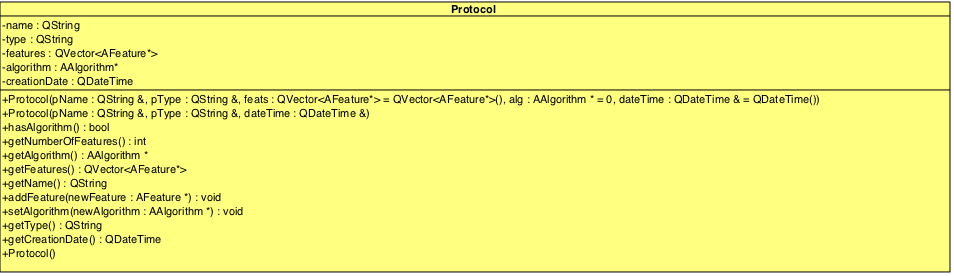
\includegraphics[scale=0.6]{./Content/Immagini/modelCore/Protocol.png}
			\caption{Diagramma classe \textsl{Protocol}}
			\label{Protocol_img}
\end{figure}

\paragraph{Descrizione \\}
Classe che rappresenta un Protocol\g{} con le relative propietà: \emph{Nome, Tipo, Data di creazione, Lista di feature\g{} e Algoritmo di cluster\g{}}.

\paragraph{Utilizzo \\}
viene utilizzata in seguito alla ricezione di un signal\g{} da parte dei controller che necessitano di riferirsi ad uno o più Protocol\g{}.
\\Inoltre viene utilizzata dalla classe \textsl{Dataset}, che contiene un riferimento ai Protocol\g{} associati, e dalle classi DAO.

\paragraph{Attributi}
	\begin{itemize}
	 	% name
		\item \color{teal}\verb!- name : QString !
		\color{black}\subparagraph{Descrizione:} nome del \protocol{}.
		
		%tpye
		\item \color{teal}\verb! -type : QString !
		\color{black}\subparagraph{Descrizione:} il tipo del Protocol\g{} (2D, 2D-t, 3D, 3D-t).
		
		% features
		\item \color{teal}\verb!- features : QVector<AFeature*> !
		\color{black} \subparagraph{Descrizione: } vettore di puntatori polimorfi ad oggetti \textsl{AFeature} contenente le feature\g{} del \protocol{}.
		
		%algorithm
		\item \color{teal}\verb!- algorithm : AAlgorithm* !
		\color{black}\subparagraph{Descrizione:} puntatore polimorfo all'algoritmo di clustering\g{}. Nel caso in cui non ci sia alcun algoritmi, \verb!algorithm! varrà 0.
		
		%date
		\item \color{teal}\verb! - creationDate : QDateTime !
		\color{black}\subparagraph{Descrizione:} data di creazione del Protocol\g{}.
		
	\end{itemize}

\color{black}
\pagebreak
\paragraph{Metodi}
	\begin{itemize}
		%costruttore
		\item \color{blue}\verb! + Protocol(pName : const QString&, pType : const QString& , feats : QVector<AFeature*>, !\\
								\verb!alg : AAlgorithm *, dateTime : const QDateTime& )!\\
				\color{black}
				\subparagraph{Descrizione:} costruttore della classe \textsl{Protocol}.
				\subparagraph{Argomenti}
					\begin{itemize}
						\item \color{RoyalPurple}\verb!pName : const QString&!\\
						\color{black}Nome del Protocol\g{};
						
						\item \color{RoyalPurple}\verb!pType : const QString&!\\
						\color{black}Tipo del Protocol\g{} (2D, 2D-t, 3D, 3D-t);
						
						\item \color{RoyalPurple}\verb!feats : QVector<AFeature*>!\\
						\color{black}Elenco di feature\g{} presenti nel Protocol\g{};
						
						\item \color{RoyalPurple}\verb!alg : AAlgorithm *!\\
						\color{black}Algoritmo di clustering\g{} presente nel Protocol\g{};
						
						\item \color{RoyalPurple}\verb!dateTime : const QDateTime&!\\
						\color{black}Data di creazione del Protocol\g{}.
					\end{itemize}
			
		\item \color{blue}\verb! + Protocol(pName : const QString&, pType :  const QString&, dateTime : const QDateTime&)!\\
			\color{black}
			\subparagraph{Descrizione:} costuttore utilizzato per creare un Protocol\g{} vuoto.
			\subparagraph{Argomenti}
				\begin{itemize}
					\item \color{RoyalPurple}\verb!pName : const QString&!\\
					\color{black}Nome del Protocol\g{};
					
					\item \color{RoyalPurple}\verb!pType :  const QString&!\\
					\color{black}Tipo del Protocol\g{} (2D, 2D-t, 3D, 3D-t).
				\end{itemize}
		
		%hasAlogrithm
		\item \color{blue}\verb! + hasAlgorithm() : boolean!\\
		\color{black}
		\subparagraph{Descrizione:} metodo che controlla se il Protocol\g{} ha un algoritmo di clustering\g{} o meno.
		\subparagraph{Note}
			\begin{itemize}
				\item Il metodo deve essere marcato come costante.
			\end{itemize}		
		
		%getNumberOfFeatures
		\item \color{blue}\verb! + getNumberOfFeatures(): int!\\
		\color{black}
		\subparagraph{Descrizione:} metodo che ritorna il numero di feature\g{} presenti nel Protocol\g{}.
		\subparagraph{Note}
			\begin{itemize}
				\item Il metodo deve essere marcato come costante.
			\end{itemize}
		
		%getAlgorithm
		\item \color{blue}\verb! + getAlgorithm() : AAlgorithm* !\\
		\color{black}
		\subparagraph{Descrizione:} ritorna il puntatore all'algoritmo di clustering\g{} del \protocol{}.
		\\S il Protocol\g{} non contiene alcun algoritmo di clsutering\g{} viene ritornato 0.
		\subparagraph{Note}
		\begin{itemize}
			\item Il metodo deve essere marcato come costante.
		\end{itemize}
		
		%getFeatures
		\item \color{blue}\verb! + getFeatures() : QVector<AFeature*> !\\
		\color{black} 
		\subparagraph{Descrizione:} ritorna un vettore di puntatori alle feature\g{} del \protocol{}.
		\subparagraph{Note}	
		\begin{itemize}
			\item Il metodo deve essere marcato come costante.
		\end{itemize}
		
		% getName
		\item \color{blue}\verb! + getName() : QString !
		\color{black}
		\subparagraph{Descrizione:} ritorna una stringa contenente il nome del \protocol{}.
		\subparagraph{Note}
			\begin{itemize}
				\item  Il metodo deve essere marcato come costante.
			\end{itemize}
		
		% addFeature
		\item \color{blue}\verb! + addFeature(newFeature : AFeature *) : void !
		\color{black}
		\subparagraph{Descrizione:} aggiunge una nuova feature\g{} al \protocol{}.
		\subparagraph{Argomenti}
			\begin{itemize}
				\item \color{RoyalPurple} \verb!newFeature : AFeature *! \\ 
				\color{Black}Puntatore alla feature\g{} da aggiungere al \protocol{}. 
			\end{itemize}
			
		% setAlgorithm
		\item \color{blue}\verb! + setAlgorithm(newAlgorithm : AAlgorithm *) : void !
		\color{black}
		\subparagraph{Descrizione:} assegna un nuovo algoritmo di clustering\g{} al \protocol{}.
		\subparagraph{Argomenti}
			\begin{itemize}
				\item \color{RoyalPurple} \verb!newAlgorithm : AAlgorithm *! \\ 
				\color{black}Puntatore al nuovo algoritmo di clustering\g{} da assegnare al \protocol{}. 
			\end{itemize}
			
		% getName
		\item \color{blue}\verb! + getType() : QString !\\
		\color{black}
		\subparagraph{Descrizione:} ritorna una stringa contenente il tipo del Protocol\g{} (2D, 2D-t, 3D, 3D-t).
		\subparagraph{Note}
			\begin{itemize}
				\item Deve essere marcato come costante.
			\end{itemize}
			
		%getCreationDate
		\item \color{blue}\verb! + getCreationDate() :QDateTime!\\
		\color{black}
		\subparagraph{Descrizione:} metodo che ritorna la data di creazione del Protool\g{}.
		\subparagraph{Note}
			\begin{itemize}
				\item Il metodo deve essere marcato come costante.
			\end{itemize}
	
	\end{itemize}





\pagebreak
% % % % % % % % % % % % % % % % % % % % % % % % % % % % % 
% % Dataset % % % % % % % % % % % % % % % % % % % % %
% % % % % % % % % % % % % % % % % % % % % % % % % % % % %
\color{black}
\subsubsection{Dataset (class)}
\label{Dataset}
\begin{figure}[!h]
\centering
			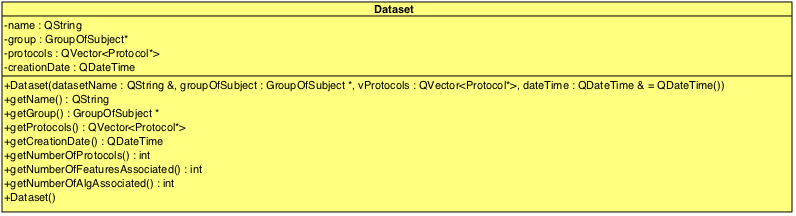
\includegraphics[scale=0.7]{./Content/Immagini/modelCore/Dataset.png}
			\caption{Diagramma classe \textsl{Dataset}}
			\label{Dataset_img}
\end{figure}

\paragraph{Descrizione \\}
Classe che rappresenta un Dataset\g{} con le relative proprietà: \textit{Nome}, \textit{Tipo}, \textit{Data di creazione}, \textit{Gruppo di Subject\g{}} e \textit{Protocol\g{}}.

\paragraph{Utilizzo \\}
Viene utilizzata in seguito alla ricezione di un signal\g{} da parte dei controller che necessitano di riferirsi ad uno o più Dataset\g{}.			
\\Inoltre viene utilizzata dalla classe \textsl{Analysis}, che contiene un riferimento al Dataset\g{} associato all'analisi, e dalle classi DAO.

\paragraph{Attributi}
	\begin{itemize}
		%name
		\item \color{blue}\verb!- name : QString !
		\color{black}
		\subparagraph{Descrizione:} nome del \dataset{}.
		
		%group
		\item \color{blue}\verb!- group : GroupOfSubject * !
		\color{black}
		\subparagraph{Descrizione:} puntatore al gruppo di Subject\g{} associato al Dataset\g{}.
	
		% protocols
		\item \color{teal}\verb!- protocol : QVector<Protocol*> !
		\color{black}
		\subparagraph{Descrizione:} vettore di puntatori a oggetti di tipo \textsl{Protocol}, contenente i vari \protocol{} presenti nel Dataset\g{}.
		
		%creationDate
		\item \color{teal}\verb! -creationDate : QDateTime !
		\color{black}
		\subparagraph{Descrizione:} data di creazione del Dataset\g{}.

	\end{itemize}

\color{black}
\paragraph{Metodi \\}
	\begin{itemize}
		%costruttore
		\item \color{blue}\verb! + Dataset(datasetName : const QString&, groupOfSubject : GroupOfSubject *,!\\
							    \verb! vProtocols : QVector<Protocol*> , dateTime :  const QDateTime&)!\\
		\color{black}
		\subparagraph{Descrizione:} costruttore della classe \textsl{Dataset}.
		\subparagraph{Argomenti}
			\begin{itemize}
				\item \color{RoyalPurple}\verb!datasetName : const QString&!\\
				\color{black}Nome del Dataset\g{};
				
				\item \color{RoyalPurple}\verb!groupOfSubject : GroupOfSubject *!\\
				\color{black}Gruppo di Subject\g{} associato al Dataset\g{};
				
				\item \color{RoyalPurple}\verb!vProtocols : QVector<Protocol*>!\\
				\color{black}Vettore di puntatori ad oggetti \textsl{Protocol} presenti nel Dataset\g{};
				
				\item \color{RoyalPurple}\verb!dateTime :  const QDateTime&!\\
				\color{black}Data di creazione del Dataset\g{}.
			\end{itemize}
		
		% getName
		\item \color{blue}\verb! + getName() : QString !\\
		\color{black}
		\subparagraph{Descrizione:} ritorna una stringa contenente il nome del \dataset{}.
		\subparagraph{Note}
			\begin{itemize}
				\item Il metodo deve essere marcato come costante.
			\end{itemize}
			
		% getGroup
		\item \color{blue}\verb! + getGroup() : GroupOfSubject * !\\
		\color{black}
		\subparagraph{Descrizione:} ritorna un puntatore al \textsl{GroupOfSubject} del Dataseet\g{}.
		\subparagraph{Note}
			\begin{itemize}
				\item Il metodo deve essere marcato come costante.
			\end{itemize}
			
		% getProtocols
		\item \color{blue}\verb! + getProtocols() : QVector<Protocol*> !\\
		\color{black}
		\subparagraph{Descrizione:} metodo che ritorna un vettore contenente i \textsl{Protocol} presenti nell'oggetto \textsl{Dataset}.
		\subparagraph{Note}
			\begin{itemize}
				\item Il metodo deve essere marcato come costante.
			\end{itemize}
		
		%getCreationDdate
		\item \color{blue}\verb! + getCreationDate() : QDateTime!\\
		\color{black}
		\subparagraph{Descrizione:} metodo che ritorna la data di creazione del Dataset\g{}.
		\subparagraph{Note}
			\begin{itemize}
				\item Il metodo deve essere marcato come costante.
			\end{itemize}
			
		%getNumberOfProtocols
		\item \color{blue}\verb! + getNumberOfProtocols() : int!\\
		\color{black}
		\subparagraph{Descrizione:} metodo che ritorna il numero di Protocol\g{} nel Dataset\g{}.
		\subparagraph{Note}
			\begin{itemize}
				\item Il metodo deve essere marcato come costante.
			\end{itemize}
			
		%getNumberOfFeaturesAssociated
		\item \color{blue}\verb! + getNumberOfFeaturesAssociated() : int!\\
		\color{black}
		\subparagraph{Descrizione:} metodo che ritorna il numero totale di feature\g{} presenti nel Dataset\g{}.
		\subparagraph{Note}
			\begin{itemize}
				\item Il metodo deve essere marcato come costante.
			\end{itemize}
			
		%getNumberofAlgAssociated
		\item \color{blue}\verb! + getNumberOfAlgAssociated() : int!\\
		\color{black}
		\subparagraph{Descrizione:} metodo che ritorna il numero totale di algoritmi di clustering\g{} presenti nel Dataset\g{}.
		\subparagraph{Note}
			\begin{itemize}
				\item il metodo deve essere marcato come costante.
			\end{itemize}
		
		
		
		
		
		
	\end{itemize}
\pagebreak
% % % % % % % % % % % % % % % % % % % % % % % % % % % % % 
% % FeatCreator % % % % % % % % % % % % % % % % % % % % %
% % % % % % % % % % % % % % % % % % % % % % % % % % % % %
\color{black}
\subsubsection{FeatCreator (class)}
\label{FeatCreator}
\begin{figure}[!h]
\centering
			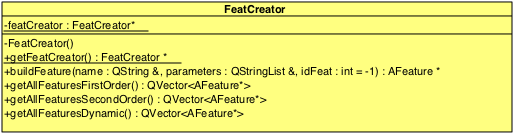
\includegraphics[scale=1]{./Content/Immagini/modelCore/FeatCreator.png}
			\caption{Diagramma classe \textsl{FeatCreator}}
			\label{FeatCreator_img}
\end{figure}

\paragraph{Descrizione \\}
Classe Factory avente la responsibilità di creare un oggetto della classe Romeo::Model::Core::Features::AFeature, che rappresenta un'istanza della feature\glossario{} da creare.
\\Rappresenta il componente Factory del design pattern\g{} Factory.
\\A seconda dei parametri e nome della Feature\g{} passati, crea un oggetto rispetto ad un altro.

\paragraph{Utilizzo \\}
Viene utilizzata in seguito alla ricezione di un signal\g{} da parte dei controller che necessitano di utilizzare un oggetto di tipo \textsl{Romeo::Model::Core::Algorithms::AFearure}.
\\A seconda dei parametri e nome della feature\g{} passati, crea un oggetto rispetto ad un altro.

\paragraph{Attributi}
	\begin{itemize}
		%featCreator
		\item \color{teal}\verb!- static featCreator: FeatCreator *!
			\color{black}
			\subparagraph{Descrizione:} puntatore all'unica istanza della classe \textsl{FeatCreator} che verrà creata in modo \textit{lazy} quando verrà richiesta la creazione dell'oggetto.
			
	\end{itemize}
	
\paragraph{Metodi}
	\begin{itemize}
		%costruttore
		\item \color{blue}\verb! + FeatCreator() !\\
		\color{black}
		\subparagraph{Descrizione:} costruttore della classe \textsl{FeatCreator}.
		
		
		\item \color{blue}\verb! + static getFeatCreator() : FeatCreator *!\\
		\color{black}
		\subparagraph{Descrizione:} metodo statico che  ritorna il puntatore all'unica istanza della classe \textsl{FeatCreator}. Nel caso in cui l'istanza non esista ancora, essa verrà creata e successivamente ritornata.
		\subparagraph{Note}
			\begin{itemize}
				\item Il metodo deve essere marcato come statico.
			\end{itemize}
			
		\item \color{blue}\verb! + buildFeature(name : const QString &, parameters : QStringList & ,!\\
				 					\verb! idFeat : int) : AFeature* !\\
		\color{black}
		\subparagraph{Descrizione:}Metodo che ha il compito di costruire la feature\g{} specificato, con i relativi parametri.\\
		Per esempio se il parametro \textit{name} è uguale a \lq\lq{}Mean\rq\rq{} allora verrà creato un oggetto \textit{MeanFeature} con i dati passati nei parametri.
		\subparagraph{Argomenti}
			\begin{itemize}
						\item \color{RoyalPurple}\verb!name : const QString&!\\
						\color{black}Stringa che rappresenta il nome della feature\g{} che si vuole creare;
						
						\item \color{RoyalPurple}\verb!parameters : const QStringList&!\\
						\color{black}Lista di stringhe che rappresenta i parametri da passare alla feature\g{} che si vuole creare;
						
						\item \color{RoyalPurple}\verb!idFeat : int!\\
						\color{black}Rappresenta l'id da associare alla feature\g{} che si vuole creare. Nel caso non venga specificato assumerà il valore di default di \lq\lq{}-1\rq\rq{} che indica che la feature\g{} non è già presente nel database.
					\end{itemize}
		\subparagraph{Note}
			\begin{itemize}
				\item Il metodo deve essere marcato come costante.
			\end{itemize}
	
	% getAllFirstOrderFeature
	\item \color{blue}\verb! + getAllFeatureFirstOrder() : QVector<AFeature *> !\\
	\color{black}
	\subparagraph{Descrizione:} metodo  che ha il compito di ritornare tutte le feature\g{} del primo ordine esistenti.
	\subparagraph{Note}
		\begin{itemize}
			\item Il metodo deve essere marcato come costante.
		\end{itemize}
		
	% getAllSecondOrderFeature
	\item \color{blue}\verb! + getAllFeatureSecondOrder() : QVector<AFeature *> !\\
		\color{black} 
		\subparagraph{Descrizione:} metodo che che ha il compito di ritornare tutte le feature\g{} del secondo ordine esistenti.
		\subparagraph{Note}
			\begin{itemize}
				\item Il metodo deve essere marcato come costante.
			\end{itemize}

	% getAllDynamicFeature
	\item \color{blue}\verb! + getAllFirsDynamicFeature() : QVector<AFeature *> !\\
		\color{black} 
		\subparagraph{Descrizione:} metodo  che ha il compito di ritornare tutte le feature\g{} del dinamiche esistenti.
		\subparagraph{Note}
			\begin{itemize}
				\item Il metodo deve essere marcato come costante.
			\end{itemize}
		
	\end{itemize}

	\pagebreak
% % % % % % % % % % % % % % % % % % % % % % % % % % % % % 
% % InternalData % % % % % % % % % % % % % % % % % % % % %
% % % % % % % % % % % % % % % % % % % % % % % % % % % % %
\color{black}
\subsubsection{InternalData (interface)}
\label{InternalData}
\begin{figure}[!h]
\centering
			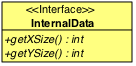
\includegraphics[scale=1]{./Content/Immagini/modelCore/InternalData.png}
			\caption{Diagramma classe \textsl{InternalData}}
			\label{InternalData_img}
\end{figure}

\paragraph{Descrizione }
Definisce l'interfaccia per accedere alle informazioni sulle dimensioni di un'immagine.
\\Rappresenta il componente Target del design pattern\g{} Adapter.

\paragraph{Utilizzo \\}
Viene utilizzata all'interno delle feature, ogni qualvolta ci si aspetta un' immagine generica.

\color{black}
\paragraph{Metodi}
	\begin{itemize}
		%getXSize
		\item \color{blue}\verb! + getXSize() : int !\\
		\color{black}
		\subparagraph{Descrizione:} contratto che ritorna la dimensione orizzantale di un'immagine generica.
		\subparagraph{Note}
			\begin{itemize}
				\item Il metodo va marcato come costante.
			\end{itemize}
			
		% getYSize	
		\item \color{blue}\verb! + getYSize() : int !
		\color{black}
		\subparagraph{Descrizione:} contratto che ritorna la dimensione verticale di un'immagine generica.
		\subparagraph{Note}
			\begin{itemize}
				\item Il metodo va marcato come costante.
			\end{itemize}

			
	\end{itemize}

\pagebreak
% % % % % % % % % % % % % % % % % % % % % % % % % % % % % 
% % InternalData2D % % % % % % % % % % % % % % % % % % % % %
% % % % % % % % % % % % % % % % % % % % % % % % % % % % %
\color{black}
\subsubsection{InternalData2D (class)}
\label{InternalData2D}
\begin{figure}[!h]
\centering
			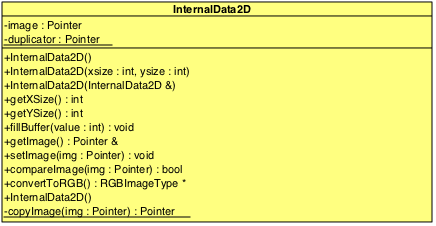
\includegraphics[scale=1]{./Content/Immagini/modelCore/InternalData2D.png}
			\caption{Diagramma classe \textsl{InternalData2D}}
			\label{InternalData2D_img}
\end{figure}

\paragraph{Descrizione\\}
Classe che implementa i contratti definiti da InternalData e rappresenta il formato interno bidimensionale sul quale operare. Implementa il design pattern Adapter e adatta la classe itk::Image della libreria ITK\g{}. Rappresenta la componente Adapter dell'omonimo design pattern\g{}.

\paragraph{Utilizzo \\}
Viene utlizzata nelle feature\g{} come parametro di input da elaborare e rappresenta i signoli canali nelle immagini in formato RGB.

\paragraph{Eredita da:}
	\begin{itemize}
		\item Romeo::Model::Core::InternalData: implementa i contratti di questa classe.
	\end{itemize}

\paragraph{Attributi}
	\begin{itemize}
		\item \color{teal}\verb! - image : ImageType2D::Pointer !\\
		\color{black}
		\subparagraph{Descrizione:} puntatore all'immagine bidimensionale (Tipo ITK\g{}).
		
		\item \color{teal}\verb! - static duplicator : DuplicatorType::Pointer!\\
		\color{black}
		\subparagraph{Desrizione:} \lq\lq{}duplicatore\rq\rq{} delle immagini \textsl{InternalData2D}.
		
	\end{itemize}
	
\paragraph{Metodi}
	\begin{itemize}
		%costruttore default
		\item \color{blue}\verb! + InternalData2D()! \\
		\color{black}
		\subparagraph{Descrizione:} costruttore di \emph{default} della lcasse \textsl{InternalData}.
		
		%costruttore
		\item \color{blue}\verb! + InternalData2D(xSize : int, ySize : int)! \\
		\color{black}
		\subparagraph{Descrizione:} costruttore a due argomenti. Costruisce un immagine di dimensioni \textit{xSize x ySize}. 
		\subparagraph{Argomenti}
			\begin{itemize}
				\item \color{RoyalPurple}\verb!xSize : int! \\ 
				\color{black}Dimensione orizzontale dell'immagine.
				
				\item \color{RoyalPurple}\verb!ySize : int! \\ 
				\color{black}Dimensione verticale dell'immagine.
			\end{itemize}
		
		%costuttore copia
		\item \color{blue}\verb! + InternalData2D(image : const InternalData &)!\\
		\color{black}
		\subparagraph{Descrizione:} costruttore di copia \emph{profondo}.
		\subparagraph{Argomenti}
			\begin{itemize}
				\item \color{RoyalPurple}\verb!image : const InternalData &!\\
				\color{black}Oggetto \textsl{InternalData2D} di cui si vuole fare la copia \emph{profonda}.
			\end{itemize}
		
		\item \color{blue}\verb! + operator=(image : const InternalData2D &) : InternalData2D&!\\
		\color{black}
		\subparagraph{Descrizione:} operatore di assegnazione \emph{profondo}.
		\subparagraph{Argomenti}
			\begin{itemize}
				\item \color{RoyalPurple}\verb!image : const InternalData &!\\
				\color{black}Oggetto \textsl{InternalData2D} di cui si vuole fare la copia \emph{profonda}.
			\end{itemize}
		
		% getXSize
		\item \color{blue}\verb! + getXSize() : int !\\
		\color{black} 
		\subparagraph{Descrizione:} implementa il contratto che ritorna la dimensione orizzontale di un'immagine.
		\subparagraph{Note}
			\begin{itemize}
				\item Il metodo deve essere marcato costante.
			\end{itemize}
		
		% getYSize
		\item \color{blue}\verb! + getYSize() : int !\\
		\color{black}
		\subparagraph{Descrizione:} implementa il contratto che ritorna la dimensione verticale di un'immagine.
		\subparagraph{Note}
			\begin{itemize}
				\item Il metodo deve essere marcato costante.
			\end{itemize}
		
		%fillBuffer
		\item \color{blue}\verb! +  fillBuffer(value : int) : void!\\
		\color{black}
		\subparagraph{Descrizione:} metodo che  \lq\lq{}riempie\rq\rq{} tutti i piexel del colore passato come argomenti.
		\subparagraph{Argomenti}
			\begin{itemize}
				\item \color{blue}\verb!value : int!\\
				\color{black}Rappresenta il colore dell'immagine (0-255). 
			\end{itemize}
		
		%getImage
		\item \color{blue}\verb! + getImage() : ImageType::Pointer& !\\
		\color{black}
		\subparagraph{Descrizione:} ritorna un puntatore ITK\g{} all'immagine rappresentata.
		
		%stImage
		\item \color{blue}\verb! + setImage(img : ImageType::Pointer) : void!\\
		\color{black}
		\subparagraph{Descrizione:} metodo che cambia l'immagine rappresentata dall'oggetto \textsl{InternalData2D}.
		\subparagraph{Argomenti}
			\begin{itemize}
				\item \color{RoyalPurple}\verb!img : ImageType::Pointer!\\
				\color{black}
				Nuova immagine da rappresentare.
			\end{itemize}
			
		\item \color{blue}\verb! + compareImage(img : ImageType::Pointer) : boolean!\\
		\color{black}
		\subparagraph{Descrizione:} metodo che controlla se due immagini sono uguali.
		\subparagraph{Argomenti}
			\begin{itemize}
				\item \color{RoyalPurple}\verb!img : ImageType::Pointer!\\
				\color{black}
				Immagine da confrontare.
			\end{itemize}
		
		%convertToRGB	
		\item \color{blue}\verb! + convertToRGB() : RGBImageType *!\\
		\color{black}
		\subparagraph{Descrizione:} metodo che converte l'oggetto \textsl{InternalData2D} in un oggetto di tipo \textsl{RGBImageType}.
		\subparagraph{Argomenti}
			\begin{itemize}
				\item Il metodo deve essere marcato costante.
			\end{itemize}
			
		% copyImage
		\item \color{blue}\verb! - static copyImage(image : ImageType2D::Pointer) : ImageType2D::Pointer !\\
		\color{black} 
		\subparagraph{Descrizione:} copia un immagine restituendone la copia.
		\subparagraph{Argomenti}
			\begin{itemize}
				\item \color{RoyalPurple}\verb!image : ImageType2D::Pointer!\\
				\color{black}Puntatore di tipo ITK\g{} all'immagine da copiare (tipo ITK\g{}).
			\end{itemize}
		\subparagraph{Note}
			\begin{itemize}
				\item Il metodo deve essere marcato come statico.
			\end{itemize}
			
	\end{itemize}
	
\pagebreak



% % % % % % % % % % % % % % % % % % % % % % % % % % % % % 
% % InternalData3D % % % % % % % % % % % % % % % % % % % % %
% % % % % % % % % % % % % % % % % % % % % % % % % % % % %
\color{black}
\subsubsection{InternalData3D (class)}
\label{InternalData3D}
\begin{figure}[!h]
\centering
			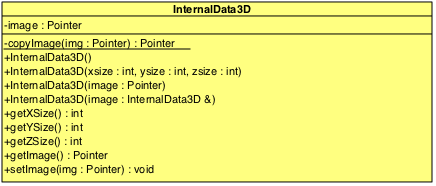
\includegraphics[scale=1]{./Content/Immagini/modelCore/InternalData3D.png}
			\caption{Diagramma Classe \textsl{InternalData3D}}
			\label{InternalData3D_img}
\end{figure}

\paragraph{Descrizione \\}
Classe che rappresenta il formato interno per un'immagine di tipo 3D.
\\Classe che \lq\lq{}adatta\rq\rq{} la classe itk::image fornita dalla libreria esterna ITK\g{}.
\\Rappresenta il componente Adapter del design pattern\g{} Adapter.

\paragraph{Utilizzo \\}
Viene utlizzata nelle feature\g{} come parametro di input da elaborare e rappresenta i signoli canali nelle immagini in formato RGB.

\paragraph{Eredita da:}
\begin{itemize}
	\item InternalData: implementa contratti di questa classe.
\end{itemize}

\paragraph{Attributi \\}
	\begin{itemize}
		\item \color{teal}\verb!- image : ImageType3D::Pointer !
		\color{black}
		\subparagraph{Descrizione:} puntatore all'immagine tridimensionale (Tipo ITK\g{}).
	\end{itemize}
	
\color{black}
\paragraph{Metodi}
	\begin{itemize}
		\item \color{blue}\verb! + InternalData3D()! 
		\color{black} 
		\subparagraph{Descrizione:} costruttore di \emph{default} della classe \textsl{InternalData3D}.

		\item \color{blue}\verb! + InternalData3D(xSize : int, ySize : int, zSize : int)! 
		\color{black} 
		\subparagraph{Descrizione:} costruttore a tre argomenti. Costruisce un immagine tridimensionale \textit{xSize x ySize x zSize}. 
		\subparagraph{Argomenti}
			\begin{itemize}
				\item \color{RoyalPurple}\verb! xSize : int! \\ 
				\color{black}Dimensione orizzontale;
				
				\item \color{RoyalPurple} \verb!ySize : int! \\ 
				\color{black}Dimensione verticale;
				
				\item \color{RoyalPurple}\verb!zSize : int! \\ 
				\color{black}Terza dimensione.
			\end{itemize}
			
		\item \color{blue}\verb! + InternalData3D(image :  RGBImageType::Pointer )!
		\color{black}
		\subparagraph{Descrizione:} costruttore che costriuisce un oggetto \textsl{InternalData3D}.
		\subparagraph{Argomenti}
			\begin{itemize}
				\item \color{RoyalPurple}\verb!image :  RGBImageType::Pointer!\\
				\color{black}Puntatore all'immagine da creare.
			\end{itemize}		
			
		\item \color{blue}\verb!InternalData3D(image : const InternalData3D &)!
		\color{black}
		\subparagraph{Descrizione:} costruttore di copia \emph{profondo}.
		\subparagraph{Argomenti}
			\begin{itemize}
				\item \color{RoyalPurple}\verb!image : const InternalData3D &!\\
				\color{black}Immagine di cui si vuole effettuare la copia.
			\end{itemize}
			
		% getXSize
		\item \color{blue}\verb! + getXSize() : int !\\
		\color{black} 
		\subparagraph{Descrizione:} implementa il contratto che ritorna la dimensione orizzontale di un'immagine.
		\subparagraph{Note}
			\begin{itemize}
				\item Il metodo deve essere marcato costante.
			\end{itemize}
		
		% getYSize
		\item \color{blue}\verb! + getYSize() : int !\\
		\color{black}
		\subparagraph{Descrizione:} implementa il contratto che ritorna la dimensione verticale di un'immagine.
		\subparagraph{Note}
			\begin{itemize}
				\item Il metodo deve essere marcato costante.
			\end{itemize}
			
		% getYSize
		\item \color{blue}\verb! + getZSize() : int !\\
		\color{black}
		\subparagraph{Descrizione:} implementa il contratto che ritorna la terza dimensione di un'immagine.
		\subparagraph{Note}
			\begin{itemize}
				\item Il metodo deve essere marcato costante.
			\end{itemize}
			
	%getImage
	\item \color{blue}\verb! + getImage() : ImageType::Pointer& !\\
	\color{black}
	\subparagraph{Descrizione:} ritorna un puntatore ITK\g{} all'immagine rappresentata.
			
	%stImage
	\item \color{blue}\verb! + setImage(img : ImageType::Pointer) : void!\\
	\color{black}
	\subparagraph{Descrizione:} metodo che cambia l'immagine rappresentata dall'oggetto \textsl{InternalData2D}.
	\subparagraph{Argomenti}
		\begin{itemize}
			\item \color{RoyalPurple}\verb!img : ImageType::Pointer!\\
			\color{black}
			Nuova immagine da rappresentare.
		\end{itemize}
		
		% copyImage
		\item \color{blue}\verb! - static copyImage(image : ImageType2D::Pointer) : ImageType2D::Pointer !\\
		\color{black} 
		\subparagraph{Descrizione:} copia un immagine restituendone la copia.
		\subparagraph{Argomenti}
			\begin{itemize}
				\item \color{RoyalPurple}\verb!image : ImageType2D::Pointer!\\
				\color{black}Puntatore di tipo ITK\g{} all'immagine da copiare (tipo ITK\g{}).
			\end{itemize}
		\subparagraph{Note}
			\begin{itemize}
				\item Il metodo deve essere marcato come statico.
			\end{itemize}
		
	\end{itemize}
	
\pagebreak	
	% % % % % % % % % % % % % % % % % % % % % % % % % % % % % %
	% % RomeoObject % % % % % % % % % % % % % % % % % % % % %
	% % % % % % % % % % % % % % % % % % % % % % % % % % % % % %
	
	\color{black}
	\subsubsection{RomeoObject(interface)}
	\label{romeoobject}
		\begin{figure}[!h]
			\centering
			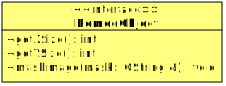
\includegraphics[scale=1]{./Content/Immagini/modelCore/RomeoObject}
			\caption{Diagramma calsse \textsl{RomeoObject}}
			\label{romeoobject_img}
		\end{figure}
		
	\paragraph{Descrizione\\}
	Intefaccia che rappresenta un generico dato da analizzare in Romeo\g{}.
	
	\paragraph{Utilizzo\\}
	Viene utilizzato nei metodi delle feature e algoritmi per lavorare su un generico dato.
	
	\paragraph{Metodi}
		\begin{itemize}
			\item \color{blue}\verb! + getXSize() : int !\\
			\color{black}
			\subparagraph{Descrione:} contratto che ritorna la dimensione x del dato.
			\subparagraph{Note}
				\begin{itemize}
					\item Il metodo deve essere marcato come costante.
				\end{itemize}
				
				\item \color{blue}\verb! + getYSize() : int !\\
					\color{black}
					\subparagraph{Descrione:} contratto che ritorna la dimensione y del dato.
					\subparagraph{Note}
						\begin{itemize}
							\item Il metodo deve essere marcato come costante.
						\end{itemize}
						
				\item \color{blue}\verb! + maskImage(mask : const QString &) : void!\\
				\color{black}
				\subparagraph{Descrizione:} contratto che applica la maschera ad un dato.
				\subparagraph{Argomenti}
					\begin{itemize}
						\item \color{RoyalPurple}\verb!mask : const QString &!\\
						\color{black}Percorso della maschera\g{} da applicare al dato. 
					\end{itemize}
				
			
		\end{itemize}
		
	
\pagebreak	

% % % % % % % % % % % % % % % % % % % % % % % % % % % % % 
% % RGBImage % % % % % % % % % % % % % % % % % % % % %
% % % % % % % % % % % % % % % % % % % % % % % % % % % % %
\color{black}
\subsubsection{RGBImage (abstract)}
\label{RGBImage}
\begin{figure}[!h]
\centering
			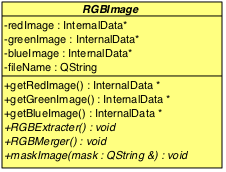
\includegraphics[scale=1]{./Content/Immagini/modelCore/RGBImage.png}
			\caption{Diagramma classe \textsl{RGBImage}}
			\label{RGBImage_img}
\end{figure}

\paragraph{Descrizione \\}
Classe astratta che rappresenta un'immagine RGB, composta da tre livelli di colore \textit{red, green} e \textit{blue}. Definisce dei contratti per l'accesso ai tre livelli di colore, per la loro scomposizione e fusione.

\paragraph{Utilizzo \\}
Viene utilizzata quando una feature\g{}  deve essere applicata ad un immagine e non ad un video.
\\Inoltre viene utilizzata per salvare le informazioni riguardanti il colore dell'immagine, che altrimenti sarebbe in scala di grigi.

\paragraph{Attributi \\}
	\begin{itemize}
		% fileName
		\item \color{teal}\verb!- fileName : QString !
		\color{black} 
		\subparagraph{Descrizione:} nome dell'immagine.
		
		% redimage
		\item \color{teal}\verb!- redImage : InternalDat a* !
		\color{black} Puntatore polimorfo al formato interno rappresentante il livello di rosso di un'immagine.

		% greenimage
		\item \color{teal}\verb!- greenImage : InternalData* !
			\color{black}
			\subparagraph{Descrizione:} puntatore polimorfo al formato interno rappresentante il livello di verde di un'immagine.
			\
			
		% blueimage
		\item \color{teal}\verb!- blueImage : InternalData* !
		\color{black} 
		\subparagraph{Descrizione:} puntatore polimorfo al formato interno rappresentante il livello di blu di un'immagine.

	\end{itemize}

\paragraph{Metodi \\}
	\begin{itemize}
	   % getRedImage
		\item \color{blue}\verb! + getRedImage() : InternalData *! 
		\color{black}
		\subparagraph{Descrizione:} metodo che ritorna il puntatore al formato interno rappresentante il livello di rosso di un'immagine.
	
		% getGreenImage
		\item \color{blue}\verb! + getGreenImage() : InternalData *!
		\color{black} 
		\subparagraph{Descrizione:} metodo che ritorna il puntatore al formato interno rappresentante il livello di verde di un'immagine.
		
		% getBlueImage
		\item \color{blue}\verb! + getBlueImage() : InternalData *! 
		\color{black} 
		\subparagraph{Descrizione;} metodo che ritorna il puntatore al formato interno rappresentante il livello di blu di un'immagine.
		
		
		% RGBExtracter
		\item \color{blue}\verb! + RGBExtracter() : void! 
		\color{black}
		\subparagraph{Descrizione:} contratto che estrae da un'immagine RGB tre formati interni rappresentanti i tre diversi livelli di un'immagine.
		
		% RGBMerger
		\item \color{blue}\verb! + RGBMerger() : void! 
		\color{black}
		\subparagraph{Descrizione:} contratto che ricompone un'immagine RGB ricostruendola dai tre formati interni rappresentanti i tre diversi livelli di un'immagine.
	\end{itemize}

	\pagebreak
% % % % % % % % % % % % % % % % % % % % % % % % % % % % % 
% % RGBImage2D % % % % % % % % % % % % % % % % % % % % %
% % % % % % % % % % % % % % % % % % % % % % % % % % % % %
\color{black}
\subsubsection{RGBImage2D (class)}
\label{RGBImage2D}
\begin{figure}[!h]
\centering
			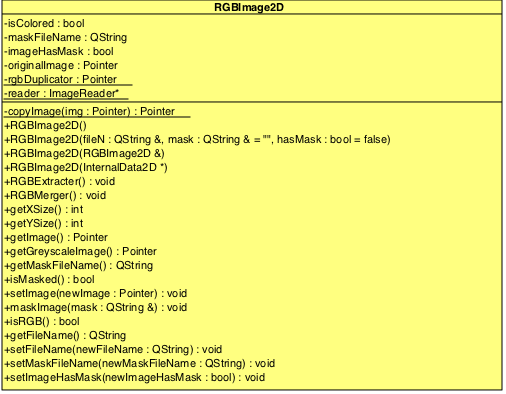
\includegraphics[scale=1]{./Content/Immagini/modelCore/RGBImage2D.png}
			\caption{Diagramma classe \textsl{ RGBImage2D}}
			\label{RGBImage2D_img}
\end{figure}

\paragraph{Descrizione \\}
Classe che rappresenta un immagine bidimensionale, a colori in Romeo\g{}
\\Classe che \lq\lq{}adatta\rq\rq{} la classe itk::image fornita da itk.
\\Rappresenta il componente Adapter del design pattern\g{} Adapter.

\paragraph{Utilizzo \\}
Viene utilizzata dalle feature\g{} che elaborano immagini bidimensionali.
\\Inoltre racchiude in se le informazioni sul colore delle immagini importate 

\paragraph{Eredita da:}
\begin{itemize}
	\item Romeo::Model::Core::RGBImage.
\end{itemize}

\paragraph{Attributi}
	\begin{itemize}
		% originalImage
		\item \color{teal}\verb!- originalImage : RGBImageType::Pointer !\\
		\color{black}
		\subparagraph{Descrizione:} puntatore all'immagine.
		
		%iscolored
		\item \color{teal}\verb! -isColored : boolean!\\
		\color{black}
		\subparagraph{Descrizione:} booleano che indica se l'immagine è colorata o a scala di grigi.
		
		%maskFileName
		\item \color{teal}\verb! - maskFileName : QString!\\
		\color{black}
		\subparagraph{Descrizione:} percorseo della maschera\g{} dell'immagine.
		
		\item \color{teal}\verb! - imageHasMask : boolean!\\
		\color{black}
		\subparagraph{Descrizione:} booelano che indica se l'immagine ha una maschera o no.
		
		\item \color{teal}\verb! -static rgbDuplicator : DuplicatorType::Pointer !\\
		\color{black}
		\subparagraph{Descrizione:} duplicatore per un immagine di tipo \textsl{RGBImage2D}.
		
		\item \color{teal}\verb! - static  reader : ImageReader*!
		\color{black}
		\subparagraph{Descrizione:} reader pr un'immagine di tipo \textsl{RGBImage2D}.
		

	\end{itemize}

\color{black}
\paragraph{Metodi }
	\begin{itemize}
	 %RGBImage2D
		\item \color{blue}\verb! + RGBImage2D()! \\
		\color{black} Costruttore di \emph{default} della classe \textsl{RGBImage2D}.
		
		% RGBImage2D
		\item \color{blue}\verb! + RGBImage2D(fileName : const QString &,  mask ; const QString&,!\\
								   \verb!hasMask : boolean)! 
			\color{black} 
			\subparagraph{Descrizione:} costruttore a tre argomenti della classe \textsl{RGBImage2D}.	
			\subparagraph{Argomenti}
			\begin{itemize}
				\item \color{RoyalPurple}\verb!fileName : QString &! \\
				\color{black}Percorso dell'immagine da caricare. Verrà passato al \textit{ReaderImage} che caricherà l'immagine.
			\end{itemize}
			
		\item \color{blue}\verb! + RGBImage2D(image : const RGBImage2D &)!\\
		\color{black}
		\subparagraph{Descrizione:} costruttore di copia \emph{profondo}.
		\subparagraph{Argomenti:}
			\begin{itemize}
				\item \color{RoyalPurple}\verb!image : const RGBImage2D &)!\\
				\color{black}Immagine di cui si vuole fare la copia.
			\end{itemize}
		
		\item \color{blue}\verb! + RGBImage2D(image : InternalData2D*)!\\
		\color{black}
		\subparagraph{Descrizione:} costruisce un'immagine \textsl{RGBImage2D} a partire da un oggetto \textsl{InternalData2D}.
		\subparagraph{Argomenti}
			\begin{itemize}
				\item \color{RoyalPurple}\verb!image : InternalData2D*!\\
				\color{black}Oggetto \textsl{InternalData2D} da cui si vuole ricavare l'oggetto \textsl{RGBImage2D}.
			\end{itemize}
			
	% RGBExtracter
		\item \color{blue}\verb! + RGBExtracter() : void! 
		\color{black}
		\subparagraph{Descrizione:} metodo che estrae da un'immagine RGB tre formati interni rappresentanti i tre diversi livelli di un'immagine.
		
		% RGBMerger
		\item \color{blue}\verb! + RGBMerger() : void! 
		\color{black}
		\subparagraph{Descrizione:} metodo che ricompone un'immagine RGB ricostruendola dai tre formati interni rappresentanti i tre diversi livelli di un'immagine.
		
	% getXSize
	\item \color{blue}\verb! + getXSize() : int !\\
	\color{black}
	\subparagraph{Descrizione: } ritorna la dimensione orizzontale dell'immagine.
	\subparagraph{Note}
		\begin{itemize}
			\item Il metodo deve essere marcato come costante.
		\end{itemize}
		
	% getYSize
	\item \color{blue}\verb! + getYSize() : int !\\
	\color{black}
	\subparagraph{Descrizione: } ritorna la dimensione verticale dell'immagine.
	\subparagraph{Note}
		\begin{itemize}
			\item Il metodo deve essere marcato come costante.
		\end{itemize}
		
	\item \color{blue}\verb! +  getImage() : RGBImageType::Pointer!\\
	\color{black}
	\subparagraph{Descrizione:} metodo che ritorna un puntatore ITK\g{} all'immagine.
	
	\item \color{blue}\verb! + getGreyscaleImage() : ImageType::Pointer!\\
	\color{black}
	\subparagraph{Descrizione:} metodo che ritorna un puntatore ITK\g{} all'immagine rappresentata come scala di grigi.
	
	\item \color{blue}\verb! + getMaskFileName() : QString!\\
	\color{black}
	\subparagraph{Descrizione:} metodo che ritorna il percorso dell'eventuale maschera\g{} dell'immagine.
	\subparagraph{Note}
		\begin{itemize}
			\item Il metodo deve essere marcato costante.
		\end{itemize}
		
	\item \color{blue}\verb! + isMasked() : boolean!\\
	\color{black}
	\subparagraph{Descrizione:} metodo che ritorna un booelano indicante se l'immagine ha una maschera o meno.
	\subparagraph{Note}
			\begin{itemize}
				\item Il metodo deve essere marcato costante.
			\end{itemize}
	
	\item \color{blue}\verb! + setImage(newImage : RGBImageType::Pointer ) : void!\\
	\color{black}
	\subparagraph{Descrizione:} metodo che cambia l'immagine rappresentata.
	\subparagraph{Argomeni}
		\begin{itemize}
			\item \color{RoyalPurple}\verb!newImage : RGBImageType::Pointer!\\
			\color{black}Puntatore ITK\g{} alla nuova immagine.
		\end{itemize}
		
	\item \color{blue}\verb! + maskImage(mask : const QString &) : void!\\
	\color{black}
	\subparagraph{Descrizione:} metodo che applica la maschera ad un immagine \textsl{RGBImage2D}.
	\subparagraph{Argomenti}
		\begin{itemize}
			\item \color{RoyalPurple}\verb!mask : const QString &!\\
			\color{black}Percorso della maschera\g{} da applicare all'oggetto \textsl{RGBImage2D}. 
		\end{itemize}
		
	\item \color{blue}\verb! + isRGB() : boolean!\\
	\color{black}
	\subparagraph{Descrizione:} metodo che ritorna un booleano indicante se l'immagine è RGB o no.
	\subparagraph{Argomenti}
		\begin{itemize}
			\item Il metodo deve essere marcato costante.
		\end{itemize}
	\subparagraph{Note}
			\begin{itemize}
				\item Il metodo deve essere marcato come costante.
			\end{itemize}
	
	\item \color{blue}\verb! + getFileName() : QString!\\
	\color{black}
	\subparagraph{Descrizione:} metodo che ritorna il nome del file rappresentato.
	\subparagraph{Note}
		\begin{itemize}
			\item Il metodo deve essere marcato come costante.
		\end{itemize}
	
	\item \color{blue}\verb! + setFileName(newFileName : QString ) : void!\\
	\color{black}
	\subparagraph{Descrizione:} metodo che cambia il file rappresentato.
	\subparagraph{Argomenti}
		\begin{itemize}
			\item \color{RoyalPurple}\verb!newFileName : QString !\\
			\color{black}Nuovo file da rappresentato.
		\end{itemize}
		
	\item \color{blue}\verb! + setMaskFileName(newMaskFileName : QString) : void!\\
	\color{black}
	\subparagraph{Descrizione:} metodo che cambia la maschera\g{} dell'immagine rappresentata.
	\subparagraph{Argomenti}
		\begin{itemize}
			\item \color{RoyalPurple}\verb!newMaskFileName : QString!\\
			\color{black}Nuova maschera.
		\end{itemize}
	  
	 \item \color{blue}\verb! +setImageHasMask(newImageHasMask : bool ) : void!\\
	  \color{black}
	  \subparagraph{Descrizione:} assegna all'attributo \verb!imageHasMask! un nuovo valore.
	  \subparagraph{Argomenti}
	  	\begin{itemize}
		  	\item \color{RoyalPurple}\verb!newImageHasMask : bool!\\
		  	\color{black}Il nuovo valore.
	  	\end{itemize}
		
		
	\end{itemize}
\pagebreak
% % % % % % % % % % % % % % % % % % % % % % % % % % % % % 
% % RGBImage3D % % % % % % % % % % % % % % % % % % % % %
% % % % % % % % % % % % % % % % % % % % % % % % % % % % %
\color{black}
\subsubsection{RGBImage3D (class)}
\label{RGBImage3D}
\begin{figure}[!h]
\centering
			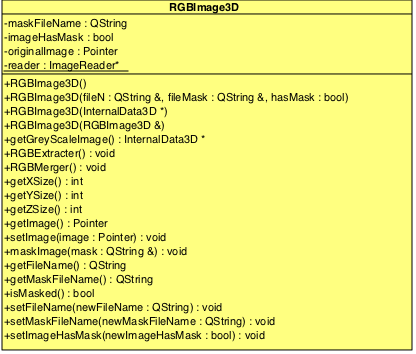
\includegraphics[scale=1]{./Content/Immagini/modelCore/RGBImage3D.png}
			\caption{Diagramma classe \textsl{RGBImage3D}}
			\label{RGBImage3D_img}
\end{figure}

\paragraph{Descrizione \\}
Classe che concretizza RGBImage e rappresenta un'immagine RGB tridimensionale, composta da tre livelli di colore \textit{red, green} e \textit{blue}. Implementa i contratti per l'accesso ai tre livelli di colore, per la loro scomposizione e fusione.
Utilizza il template itk::Image della libreria ITK\g{} per rappresentare l'immagine.

\paragraph{Utilizzo \\}
Viene utilizzata dalle sottoclassi di AFeature e di AAlgorithm per applicare le varie feature\g{} e algoritmi di clustering\g{}.

\paragraph{Eredita da:}
\begin{itemize}
	\item Romeo::Model::Core::RGBImage.
\end{itemize}

\paragraph{Attributi}
	\begin{itemize}
		% originalImage
		\item \color{teal}\verb!- originalImage : RGBImageType::Pointer !\\
		\color{black}
		\subparagraph{Descrizione:} puntatore all'immagine.
		
		
		
		%maskFileName
		\item \color{teal}\verb! - maskFileName : QString!\\
		\color{black}
		\subparagraph{Descrizione:} percorseo della maschera\g{} dell'immagine.
		
		\item \color{teal}\verb! - imageHasMask : boolean!\\
		\color{black}
		\subparagraph{Descrizione:} booelano che indica se l'immagine ha una maschera o no.
		
		\item \color{teal}\verb! - static  reader : ImageReader*!
		\color{black}
		\subparagraph{Descrizione:} reader pr un'immagine di tipo \textsl{RGBImage3D}.
		

	\end{itemize}

\color{black}
\paragraph{Metodi }
	\begin{itemize}
	 %RGBImage2D
		\item \color{blue}\verb! + RGBImage3D()! \\
		\color{black} Costruttore di \emph{default} della classe \textsl{RGBImage3D}.
		
		% RGBImage2D
		\item \color{blue}\verb! + RGBImage3D(fileName : const QString &,  mask ; const QString&,!\\
								   \verb!hasMask : boolean)! 
			\color{black} 
			\subparagraph{Descrizione:} costruttore a tre argomenti della classe \textsl{RGBImage3D}.	
			\subparagraph{Argomenti}
			\begin{itemize}
				\item \color{RoyalPurple}\verb!fileName : QString &! \\
				\color{black}Percorso dell'immagine da caricare. Verrà passato al \textit{ReaderImage} che caricherà l'immagine.
			\end{itemize}
			
		\item \color{blue}\verb! + RGBImage3D(image : const RGBImage3D &)!\\
		\color{black}
		\subparagraph{Descrizione:} costruttore di copia \emph{profondo}.
		\subparagraph{Argomenti:}
			\begin{itemize}
				\item \color{RoyalPurple}\verb!image : const RGBImag3D &)!\\
				\color{black}Immagine di cui si vuole fare la copia.
			\end{itemize}
		
		\item \color{blue}\verb! + RGBImage3D(image : InternalData3D*)!\\
		\color{black}
		\subparagraph{Descrizione:} costruisce un'immagine \textsl{RGBImage3D} a partire da un oggetto \textsl{InternalData3D}.
		\subparagraph{Argomenti}
			\begin{itemize}
				\item \color{RoyalPurple}\verb!image : InternalData3D*!\\
				\color{black}Oggetto \textsl{InternalDat3D} da cui si vuole ricavare l'oggetto \textsl{RGBImage3D}.
			\end{itemize}
			
	% RGBExtracter
		\item \color{blue}\verb! + RGBExtracter() : void! 
		\color{black}
		\subparagraph{Descrizione:} metodo che estrae da un'immagine RGB tre formati interni rappresentanti i tre diversi livelli di un'immagine.
		
		% RGBMerger
		\item \color{blue}\verb! + RGBMerger() : void! 
		\color{black}
		\subparagraph{Descrizione:} metodo che ricompone un'immagine RGB ricostruendola dai tre formati interni rappresentanti i tre diversi livelli di un'immagine.
		
	% getXSize
	\item \color{blue}\verb! + getXSize() : int !\\
	\color{black}
	\subparagraph{Descrizione: } ritorna la dimensione orizzontale dell'immagine.
	\subparagraph{Note}
		\begin{itemize}
			\item Il metodo deve essere marcato come costante.
		\end{itemize}
		
	% getYSize
	\item \color{blue}\verb! + getYSize() : int !\\
	\color{black}
	\subparagraph{Descrizione: } ritorna la dimensione verticale dell'immagine.
	\subparagraph{Note}
		\begin{itemize}
			\item Il metodo deve essere marcato come costante.
		\end{itemize}
	
	%getZSize
	\item \color{blue}\verb! + getZSize() : int!\\
	\color{black}
	\subparagraph{Descrizione:} ritorna la terza  dimensione dell'immagine.
	\subparagraph{Note}
		\begin{itemize}
			\item Il metodo deve essere marcato come costante.
		\end{itemize}
		
	\item \color{blue}\verb! +  getImage() : RGBImageType::Pointer!\\
	\color{black}
	\subparagraph{Descrizione:} metodo che ritorna un puntatore ITK\g{} all'immagine.
	
	\item \color{blue}\verb! + getGreyscaleImage() : ImageType::Pointer!\\
	\color{black}
	\subparagraph{Descrizione:} metodo che ritorna un puntatore ITK\g{} all'immagine rappresentata come scala di grigi.
	
	\item \color{blue}\verb! + getMaskFileName() : QString!\\
	\color{black}
	\subparagraph{Descrizione:} metodo che ritorna il percorso dell'eventuale maschera\g{} dell'immagine.
	\subparagraph{Note}
		\begin{itemize}
			\item Il metodo deve essere marcato costante.
		\end{itemize}
		
	\item \color{blue}\verb! + isMasked() : boolean!\\
	\color{black}
	\subparagraph{Descrizione:} metodo che ritorna un booelano indicante se l'immagine ha una maschera o meno.
	\subparagraph{Note}
			\begin{itemize}
				\item Il metodo deve essere marcato costante.
			\end{itemize}
	
	\item \color{blue}\verb! + setImage(newImage : RGBImageType::Pointer ) : void!\\
	\color{black}
	\subparagraph{Descrizione:} metodo che cambia l'immagine rappresentata.
	\subparagraph{Argomeni}
		\begin{itemize}
			\item \color{RoyalPurple}\verb!newImage : RGBImageType::Pointer!\\
			\color{black}Puntatore ITK\g{} alla nuova immagine.
		\end{itemize}
		
	\item \color{blue}\verb! + maskImage(mask : const QString &) : void!\\
	\color{black}
	\subparagraph{Descrizione:} metodo che applica la maschera ad un immagine \textsl{RGBImage3D}.
	\subparagraph{Argomenti}
		\begin{itemize}
			\item \color{RoyalPurple}\verb!mask : const QString &!\\
			\color{black}Percorso della maschera\g{} da applicare all'oggetto \textsl{RGBImage3D}. 
		\end{itemize}
		
	\item \color{blue}\verb! + isRGB() : boolean!\\
	\color{black}
	\subparagraph{Descrizione:} metodo che ritorna un booleano indicante se l'immagine è RGB o no.
	\subparagraph{Argomenti}
	\subparagraph{Note}
			\begin{itemize}
				\item Il metodo deve essere marcato come costante.
			\end{itemize}
	
	\item \color{blue}\verb! + getFileName() : QString!\\
	\color{black}
	\subparagraph{Descrizione:} metodo che ritorna il nome del file rappresentato.
	\subparagraph{Note}
		\begin{itemize}
			\item Il metodo deve essere marcato come costante.
		\end{itemize}
	
	\item \color{blue}\verb! + setFileName(newFileName : QString ) : void!\\
	\color{black}
	\subparagraph{Descrizione:} metodo che cambia il file rappresentato.
	\subparagraph{Argomenti}
		\begin{itemize}
			\item \color{RoyalPurple}\verb!newFileName : QString !\\
			\color{black}Nuovo file da rappresentato.
		\end{itemize}
		
	\item \color{blue}\verb! + setMaskFileName(newMaskFileName : QString) : void!\\
	\color{black}
	\subparagraph{Descrizione:} metodo che cambia la maschera\g{} dell'immagine rappresentata.
	\subparagraph{Argomenti}
		\begin{itemize}
			\item \color{RoyalPurple}\verb!newMaskFileName : QString!\\
			\color{black}Nuova maschera.
		\end{itemize}
	  
	 \item \color{blue}\verb! +setImageHasMask(newImageHasMask : bool ) : void!\\
	  \color{black}
	  \subparagraph{Descrizione:} assegna all'attributo \verb!imageHasMask! un nuovo valore.
	  \subparagraph{Argomenti}
	  	\begin{itemize}
		  	\item \color{RoyalPurple}\verb!newImageHasMask : bool!\\
		  	\color{black}Il nuovo valore.
	  	\end{itemize}
	
	\end{itemize}

% % % % % % % % % % % % % % % % % % % % % % % % % % % % % 
% % Video % % % % % % % % % % % % % % % % % % % % %
% % % % % % % % % % % % % % % % % % % % % % % % % % % % %
\pagebreak
\subsubsection{Video(abstract)}
\label{Video}
\begin{figure}[!h]
\centering
			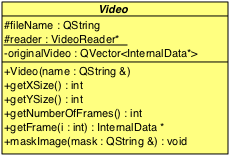
\includegraphics[scale=1]{./Content/Immagini/modelCore/Video.png}
			\caption{Diagramma classe \textsl{Video}}
			\label{RGBVideo_img}
\end{figure}

\paragraph{Descrizione \\}
Classe astratta che rappresenta la classe base di tutti i video in Romeo\g{}.
\\È composta da un vettore di oggetti di tipo \textsl{InternalData}.

\paragraph{Utilizzo \\}
viene utilizzata dalle Feature\g{} dinamiche quando ci si aspetta un video generico.

\paragraph{Attributi\\}
	\begin{itemize}
		\item  \color{teal}\verb! # fileName : QString!\\
		\color{black}
		\subparagraph{Descrizione:} percorso del video.
		 
		 \item \color{teal}\verb! # static reader : VideoReader *!\\
		 \color{black}
		 \subparagraph{Descrizione:} puntatore al reader dei video.
		 
		 \item \color{teal}\verb! -originalVideo : QVector<InternalData *>!\\
		 \color{black}
		 \subparagraph{Descrizione:} vettore di frames del video.
	\end{itemize}
	
\paragraph{Metodi\\}
	\begin{itemize}
		\item \color{blue}\verb! + Video(name : const QStirng &)!\\
			\color{black}
			\subparagraph{Descrizione:} costruttore della classe.
			\subparagraph{Argomenti}
				\begin{itemize}
					\item \color{RoyalPurple}\verb!name : const QStirng &!\\
					\color{black}Percorso del video.
				\end{itemize}
			
		\item \color{blue}\verb! + getXSize() : int !\\
		\color{black}
		\subparagraph{Descrizione:} metodo che ritorna la larghezza del frame video.
		\subparagraph{Note}
			\begin{itemize}
				\item Il metodo deve essere marcato come costante.
			\end{itemize}
		
		\item \color{blue}\verb! + getYSize() : int !\\
		\color{black}
		\subparagraph{Descrizione:} metodo che ritorna l'altezza del frame video.
		\subparagraph{Note}
			\begin{itemize}
				\item Il metodo deve essere marcato come costante.
			\end{itemize}
			
		\item \color{blue}\verb! + getNumberOfFrames() : int !\\
		\color{black}
		\subparagraph{Descrizione:} metodo che ritorna il numero di frame presenti nel video.
		\subparagraph{Note}
			\begin{itemize}
				\item Il metodo deve essere marcato come costante.
			\end{itemize}
			
		\item \color{blue}\verb! + getFrame(i : int) : InternalData * !\\
		\color{black}
		\subparagraph{Descrizione:} metodo che ritorna il frame i-esimo del video.
		\subparagraph{Argomenti}
				\begin{itemize}
					\item \color{RoyalPurple}\verb!i : int !\\
					\color{black}Indice del frame da ottenere.
				\end{itemize}
		
		\item \color{blue}\verb! + maskImage(mask : QString &) : void !\\
		\color{black}
		\subparagraph{Descrizione:} metodo che aggiunge una maschera ad un video.
		\subparagraph{Argomenti}
				\begin{itemize}
					\item \color{RoyalPurple}\verb!mask : QString & !\\
					\color{black}Percorso della maschera nel filesystem.
				\end{itemize}
		
	\end{itemize}
	
% % % % % % % % % % % % % % % % % % % % % % % % % % % % % 
% % Video2D % % % % % % % % % % % % % % % % % % % % % % %
% % % % % % % % % % % % % % % % % % % % % % % % % % % % %
\pagebreak
\subsubsection{Video2D(class)}
\label{Video2D}
\begin{figure}[!h]
\centering
			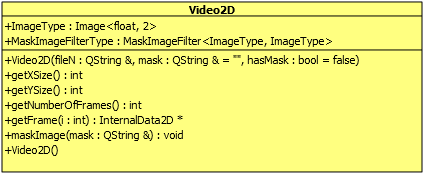
\includegraphics[scale=1]{./Content/Immagini/modelCore/Video2D.png}
			\caption{Diagramma classe \textsl{Video2D}}
			\label{Video2D_img}
\end{figure}

\paragraph{Descrizione \\}
Classe che rappresenta un video bidimensionale in Romeo\g{}.
\\È composta da un vettore di oggetti di tipo \textsl{InternalData2D}.

\paragraph{Utilizzo \\}
viene utilizzata dalle Feature\g{} dinamiche quando ci si aspetta un video bidimensionale.

\paragraph{Metodi\\}
	\begin{itemize}
		\item \color{blue}\verb! + Video2D(fileN : const QString& fileN, mask : const QString & , hasMask : bool)!\\
			\color{black}
			\subparagraph{Descrizione:} costruttore della classe.
			\subparagraph{Argomenti}
				\begin{itemize}
					\item \color{RoyalPurple}\verb!fileN : const QStirng &!\\
					\color{black}Percorso del video nel filesystem.
					\item \color{RoyalPurple}\verb!mask : const QStirng &!\\
					\color{black}Percorso della maschera del video nel filesystem.
					\item \color{RoyalPurple}\verb!hasMask : bool!\\
					\color{black} true se il video possiede una maschera.
				\end{itemize}
				
		\item \color{blue}\verb! + getXSize() : int !\\
		\color{black}
		\subparagraph{Descrizione:} metodo che ritorna la larghezza del frame video.
		\subparagraph{Note}
			\begin{itemize}
				\item Il metodo deve essere marcato come costante.
			\end{itemize}
		
		\item \color{blue}\verb! + getYSize() : int !\\
		\color{black}
		\subparagraph{Descrizione:} metodo che ritorna l'altezza del frame video.
		\subparagraph{Note}
			\begin{itemize}
				\item Il metodo deve essere marcato come costante.
			\end{itemize}
			
		\item \color{blue}\verb! + getNumberOfFrames() : int !\\
		\color{black}
		\subparagraph{Descrizione:} metodo che ritorna il numero di frame presenti nel video.
		\subparagraph{Note}
			\begin{itemize}
				\item Il metodo deve essere marcato come costante.
			\end{itemize}
			
		\item \color{blue}\verb! + getFrame(i : int) : InternalData2D * !\\
		\color{black}
		\subparagraph{Descrizione:} metodo che ritorna il frame i-esimo del video.
		\subparagraph{Argomenti}
				\begin{itemize}
					\item \color{RoyalPurple}\verb!i : int !\\
					\color{black}Indice del frame da ottenere.
				\end{itemize}
		
		\item \color{blue}\verb! + maskImage(mask : QString &) : void !\\
		\color{black}
		\subparagraph{Descrizione:} metodo che aggiunge una maschera ad un video.
		\subparagraph{Argomenti}
				\begin{itemize}
					\item \color{RoyalPurple}\verb!mask : QString & !\\
					\color{black}Percorso della maschera nel filesystem.
				\end{itemize}
				
	\end{itemize}
	
% % % % % % % % % % % % % % % % % % % % % % % % % % % % % 
% % Video3D % % % % % % % % % % % % % % % % % % % % % % %
% % % % % % % % % % % % % % % % % % % % % % % % % % % % %
\pagebreak
\subsubsection{Video3D(class)}
\label{Video3D}
\begin{figure}[!h]
\centering
			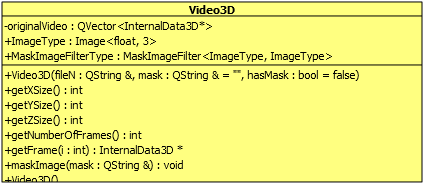
\includegraphics[scale=1]{./Content/Immagini/modelCore/Video3D.png}
			\caption{Diagramma classe \textsl{Video3D}}
			\label{Video3D_img}
\end{figure}

\paragraph{Descrizione \\}
Classe che rappresenta un video tridimensionale in Romeo\g{}.
\\È composta da un vettore di oggetti di tipo \textsl{InternalData2D}.

\paragraph{Utilizzo \\}
Viene utilizzata dalle Feature\g{} dinamiche quando ci si aspetta un video tridimensionale.

\paragraph{Metodi\\}
	\begin{itemize}
		\item \color{blue}\verb! + Video2D(fileN : const QString& fileN, mask : const QString & , hasMask : bool)!\\
			\color{black}
			\subparagraph{Descrizione:} costruttore della classe.
			\subparagraph{Argomenti}
				\begin{itemize}
					\item \color{RoyalPurple}\verb!fileN : const QStirng &!\\
					\color{black}Percorso del video nel filesystem.
					\item \color{RoyalPurple}\verb!mask : const QStirng &!\\
					\color{black}Percorso della maschera del video nel filesystem.
					\item \color{RoyalPurple}\verb!hasMask : bool!\\
					\color{black} true se il video possiede una maschera.
				\end{itemize}
				
		\item \color{blue}\verb! + getXSize() : int !\\
		\color{black}
		\subparagraph{Descrizione:} metodo che ritorna la larghezza del frame video.
		\subparagraph{Note}
			\begin{itemize}
				\item Il metodo deve essere marcato come costante.
			\end{itemize}
		
		\item \color{blue}\verb! + getYSize() : int !\\
		\color{black}
		\subparagraph{Descrizione:} metodo che ritorna l'altezza del frame video.
		\subparagraph{Note}
			\begin{itemize}
				\item Il metodo deve essere marcato come costante.
			\end{itemize}
		
		\item \color{blue}\verb! + getZSize() : int !\\
		\color{black}
		\subparagraph{Descrizione:} metodo che ritorna la profondità del frame video.
		\subparagraph{Note}
			\begin{itemize}
				\item Il metodo deve essere marcato come costante.
			\end{itemize}
			
		\item \color{blue}\verb! + getNumberOfFrames() : int !\\
		\color{black}
		\subparagraph{Descrizione:} metodo che ritorna il numero di frame presenti nel video.
		\subparagraph{Note}
			\begin{itemize}
				\item Il metodo deve essere marcato come costante.
			\end{itemize}
			
		\item \color{blue}\verb! + getFrame(i : int) : InternalData3D * !\\
		\color{black}
		\subparagraph{Descrizione:} metodo che ritorna il frame i-esimo del video.
		\subparagraph{Argomenti}
				\begin{itemize}
					\item \color{RoyalPurple}\verb!i : int !\\
					\color{black}Indice del frame da ottenere.
				\end{itemize}
		
		\item \color{blue}\verb! + maskImage(mask : QString &) : void !\\
		\color{black}
		\subparagraph{Descrizione:} metodo che aggiunge una maschera ad un video.
		\subparagraph{Argomenti}
				\begin{itemize}
					\item \color{RoyalPurple}\verb!mask : QString & !\\
					\color{black}Percorso della maschera nel filesystem.
				\end{itemize}
				
	\end{itemize}

